%%%%%%%%%%%%%%%%%%%%%%%%%%%%%%%%%%%%%%%%%%%%%%%%%%%%%%%%%%%%%%%%%%%%%%%%%
%  Content: Main file of thesis template (master/enginering).
%  Author: Tomasz Kubik <tomasz.kubik@pwr.edu.pl>
%  Data: 1 marca 2020
%  Wersja: 0.4
%%%%%%%%%%%%%%%%%%%%%%%%%%%%%%%%%%%%%%%%%%%%%%%%%%%%%%%%%%%%%%%%%%%%%%%%%

\documentclass[a4paper,onecolumn,oneside,12pt,extrafontsizes]{memoir}
% In order to prepare the manuscript for archives (2x1, double printed) you can:
% a) produce normal pdf, then convert it to pdf with two pages on one phisical page (solution suggested)
%
%   This can be done by:
%   - printing from Adobe Acrobat Reader with option "Multiple"
%   - using psutils
%
%      Windows (assuming that you have MiKTeX installed with the package pakiet miktex-psutils-bin-x64-2.9):
%        "c:\Program Files\MiKTeX 2.9\miktex\bin\x64\pdf2ps.exe" Dyplom.pdf Dyplom.ps
%        "c:\Program Files\MiKTeX 2.9\miktex\bin\x64\psnup.exe" -2 Dyplom.ps Dyplom2.ps
%        "c:\Program Files\MiKTeX 2.9\miktex\bin\x64\ps2pdf.exe" Dyplom2.ps Dyplom2.pdf
%        Del Dyplom2.ps Dyplom.ps
%
%     Linux:
%        pdf2ps Dyplom.pdf - | psnup -2 | ps2pdf - Dyplom2.pdf
%
%
% b) produce 'reduced' pdf by settning smaller fonts in the document class definition (it changes the formating thus it is not suggested)
%
%   Use of the following commands instead of original one:
%   \documentclass[a4paper,onecolumn,twoside,10pt]{memoir} 
%   \renewcommand{\normalsize}{\fontsize{8pt}{10pt}\selectfont}

%\usepackage[cp1250]{inputenc} % for cp1250 file encoding
\usepackage{amssymb}

\usepackage[utf8]{inputenc} % for UTF8 file encoding
\usepackage[T1]{fontenc}
\usepackage[polish]{babel}
%\usepackage[english]{babel}
%\DisemulatePackage{setspace}
\usepackage{setspace}
\usepackage{tabularx}
\usepackage{color,calc}

%\usepackage{soul} % packege with commands for text highliting

%% Accorging to the rules the main font of the thesis should be Times.
%% In order to achieve it we use tgtermes font that offers shapes: normal, bold, italic, italic bold.
%% There is no slanted shape.
%% If you use slanted font in the text (typing \textsl{} commnand), then LaTeX will substitute it with a standard font giving you a warning.
%% Additionally tgtermes works for the running text. All maths (formulas, equations) will be rendered with a default font for math.
%% If you with to change the font for math, you must to do it yourself.

%% After installation of tgtermes package there might be a need to update font and mapping information 
%% This can be don by running the following commands (as administrator)
%% initexmf --admin --update-fndb
%% initexmf --admin --mkmaps

\usepackage{tgtermes}   

\renewcommand*\ttdefault{txtt}

% The settings regarding fonts were used in the earlier version of the template. It is kept for historical reasons
%\usepackage{mathptmx} 
%\usepackage{newtxtext,newtxmath} 
%\usepackage{newtxmath,tgtermes} 

\usepackage{listings} % used to render the source code 
% In UTF8 encoding there was a need to define the following mapping (otherwise the national characters were not recognized correctly)
%%\lstset{literate=%-
%%{ą}{{\k{a}}}1 {ć}{{\'c}}1 {ę}{{\k{e}}}1 {ł}{{\l{}}}1 {ń}{{\'n}}1 {ó}{{\'o}}1 {ś}{{\'s}}1 {ż}{{\.z}}1 {ź}{{\'z}}1 {Ą}{{\k{A}}}1 {Ć}{{\'C}}1 {Ę}{{\k{E}}}1 {Ł}{{\L{}}}1 {Ń}{{\'N}}1 {Ó}{{\'O}}1 {Ś}{{\'S}}1 {Ż}{{\.Z}}1 {Ź}{{\'Z}}1 
    %%{Ö}{{\"O}}1
    %%{Ä}{{\"A}}1
    %%{Ü}{{\"U}}1
    %%{ß}{{\ss}}1
    %%{ü}{{\"u}}1
    %%{ä}{{\"a}}1
    %%{ö}{{\"o}}1
    %%{~}{{\textasciitilde}}1
		%%{—}{{{\textemdash} }}1
%%}%{\ \ }{{\ }}1}

\usepackage{pgfplots}

\usepackage{amsmath}
\usepackage{multicol}
\usepackage{placeins}

\usepackage{siunitx}
\usepackage{physics}
\usepackage[f]{esvect}
\newcommand{\normalize}[1]{
  \ensuremath{\frac{#1}{\Vert#1\Vert}}
}
\newcommand{\length}[1]{
  \ensuremath{\Vert#1\Vert}
}

\usepackage{tikz}
\usetikzlibrary{quotes,babel,calc,patterns,angles, arrows.meta, intersections}
 \usepackage{pdfpages}

 \usepackage{float}
 \usepackage{longtable}
 \usepackage{xltabular}
 \usepackage{eqexpl}
 \eqexplSetIntro{gdzie:}
% \usepackage{mathdots}
% \usepackage{yhmath}
% \usepackage{cancel}
% \usepackage{color}
% \usepackage{siunitx}
% \usepackage{array}
% \usepackage{multirow}
% \usepackage{amssymb}
% \usepackage{gensymb}
% \usepackage{tabularx}
% \usepackage{booktabs}
% \usetikzlibrary{patterns}
% \usetikzlibrary{shadows.blur}
% \usetikzlibrary{shapes}



\newcommand{\listingcaption}[1]% added to handle captions of listings in two columns 
{%
\vspace*{\abovecaptionskip}\small 
\refstepcounter{lstlisting}\hfill%
Listing \thelstlisting: #1\hfill%\hfill%
\addcontentsline{lol}{lstlisting}{\protect\numberline{\thelstlisting}#1}
}%

\lstdefinelanguage{JavaScript}{
  keywords={typeof, new, true, false, catch, function, return, null, catch, switch, var, if, in, while, do, else, case, break},
  keywordstyle=\color{blue}\bfseries,
  ndkeywords={class, export, boolean, default, extends throw, implements, import, this, void, number, string, public, private, protected, extends, from, constructor},
  ndkeywordstyle=\color{darkgray}\bfseries,
  identifierstyle=\color{black},
  sensitive=false,
  comment=[l]{//},
  morecomment=[s]{/*}{*/},
  commentstyle=\color{purple}\ttfamily,
  stringstyle=\color{red}\ttfamily,
  morestring=[b]',
  morestring=[b]"
}

% code style with line numbering (but these are commented out)
\lstset{
  basicstyle=\footnotesize\ttfamily,
  %%columns=fullflexible,
	%%showstringspaces=false,
	%%showspaces=false,
  breaklines=true,
  postbreak=\mbox{\textcolor{red}{$\hookrightarrow$}\space},
  %%numbers=left,
  %%firstnumber=1,
  %%numberfirstline=true,
	%%xleftmargin=17pt,
  %%framexleftmargin=17pt,
  %%framexrightmargin=5pt,
  %%framexbottommargin=4pt,
	belowskip=.5\baselineskip
}

% code style without line numbering
%%\lstset{
  %%basicstyle=\footnotesize\ttfamily,
  %%columns=fullflexible,
	%%showstringspaces=false,
	%%showspaces=false,
  %%breaklines=true,
  %%postbreak=\mbox{\textcolor{red}{$\hookrightarrow$}\space},
%%}

%% Here you have another example of code styling
%%\lstloadlanguages{% Check Dokumentation for further languages ...
%%C,
%%C++,
%%csh,
%%Java
%%}
%%
%%\definecolor{red}{rgb}{0.6,0,0} % for strings
%%\definecolor{blue}{rgb}{0,0,0.6}
%%\definecolor{green}{rgb}{0,0.8,0}
%%\definecolor{cyan}{rgb}{0.0,0.6,0.6}
%%
%%\lstdefinestyle{sqlstyle}{
%%language=SQL,
%%basicstyle=\footnotesize\ttfamily, 
%%numbers=left, 
%%numberstyle=\tiny, 
%%numbersep=5pt, 
%%tabsize=2, 
%%extendedchars=true, 
%%breaklines=true, 
%%showspaces=false, 
%%showtabs=true, 
%%xleftmargin=17pt,
%%framexleftmargin=17pt,
%%framexrightmargin=5pt,
%%framexbottommargin=4pt,
%%keywordstyle=\color{blue}, 
%%commentstyle=\color{green}, 
%%stringstyle=\color{red}, 
%%}
%%
%%\lstdefinestyle{sharpcstyle}{
%%language=[Sharp]C,
%%basicstyle=\footnotesize\ttfamily, 
%%numbers=left, 
%%numberstyle=\tiny, 
%%numbersep=5pt, 
%%tabsize=2, 
%%extendedchars=true, 
%%breaklines=true, 
%%showspaces=false, 
%%showtabs=true, 
%%xleftmargin=17pt,
%%framexleftmargin=17pt,
%%framexrightmargin=5pt,
%%framexbottommargin=4pt,
%%morecomment=[l]{//}, %use comment-line-style!
%%morecomment=[s]{/*}{*/}, %for multiline comments
%%showstringspaces=false, 
%%morekeywords={  abstract, event, new, struct,
                %%as, explicit, null, switch,
                %%base, extern, object, this,
                %%bool, false, operator, throw,
                %%break, finally, out, true,
                %%byte, fixed, override, try,
                %%case, float, params, typeof,
                %%catch, for, private, uint,
                %%char, foreach, protected, ulong,
                %%checked, goto, public, unchecked,
                %%class, if, readonly, unsafe,
                %%const, implicit, ref, ushort,
                %%continue, in, return, using,
                %%decimal, int, sbyte, virtual,
                %%default, interface, sealed, volatile,
                %%delegate, internal, short, void,
                %%do, is, sizeof, while,
                %%double, lock, stackalloc,
                %%else, long, static,
                %%enum, namespace, string},
%%keywordstyle=\color{cyan},
%%identifierstyle=\color{red},
%%stringstyle=\color{blue}, 
%%commentstyle=\color{green},
%%}


\renewcommand\lstlistlistingname{Spis listingów}
\makeatletter
%\renewcommand*{\l@lstlisting}[2]{\@dottedtocline{1}{0em}{2.3em}{#1}{#2}}
\g@addto@macro\insertchapterspace{\addtocontents{lol}{\protect\addvspace{10pt}}}
\renewcommand*{\l@lstlisting}{\@dottedtocline{1}{0em}{2.3em}}
\makeatother

\renewcommand*{\lstlistlistingname}{Spis listingów} \newlistof{lstlistoflistings}{lol}{\lstlistlistingname}



% It is possible to use packages mentioned below for making various tables but it is suggested to left them unused
%\usepackage{longtable}
%\usepackage{ltxtable}
%\usepackage{tabulary}

%%%%%%%%%%%%%%%%%%%%%%%%%%%%%%%%%%%%%%%%%%%%%%%%%%%
%% Settings related to the autmatic document typesetting
%% and floats placements
%%%%%%%%%%%%%%%%%%%%%%%%%%%%%%%%%%%%%%%%%%%%%%%%%%%
%\hyphenpenalty=10000		% do not break words too often
\clubpenalty=10000      % penalty for orphans
\widowpenalty=10000  % do not left widows
%\brokenpenalty=10000		% dont break words between pages - commented out because interfere with line breaking in lstlisting
%\exhyphenpenalty=999999		% dont break word with dash - commented out because interfere with line breaking in lstlisting
\righthyphenmin=3			% break at min 3 characters

%\tolerance=4500
%\pretolerance=250
%\hfuzz=1.5pt
%\hbadness=1450

\renewcommand{\topfraction}{0.95}
\renewcommand{\bottomfraction}{0.95}
\renewcommand{\textfraction}{0.05}
\renewcommand{\floatpagefraction}{0.35}

%%%%%%%%%%%%%%%%%%%%%%%%%%%%%%%%%%%%%%%%%%%%%%%%%%%
%%  Size settings: text, header and footer, marigins
%%  for documents based on memoir class
%%%%%%%%%%%%%%%%%%%%%%%%%%%%%%%%%%%%%%%%%%%%%%%%%%%
\setlength{\headsep}{10pt} 
\setlength{\headheight}{13.6pt} % baselineskip for 11pt font, i.e. \small, equals 13.6pt
\setlength{\footskip}{\headsep+\headheight}
\setlength{\uppermargin}{\headheight+\headsep+1cm}
\setlength{\textheight}{\paperheight-\uppermargin-\footskip-1.5cm}
\setlength{\textwidth}{\paperwidth-5cm}
\setlength{\spinemargin}{2.5cm}
\setlength{\foremargin}{2.5cm}
\setlength{\marginparsep}{2mm}
\setlength{\marginparwidth}{2.3mm}
%\settrimmedsize{297mm}{210mm}{*}
%\settrims{0mm}{0mm}	
\checkandfixthelayout[fixed] % needed to fix the layout
%%%%%%%%%%%%%%%%%%%%%%%%%%%%%%%%%%%%%%%%%%%%%%%%
%%  Settings related to the interline spaces, indentations, distances
%%%%%%%%%%%%%%%%%%%%%%%%%%%%%%%%%%%%%%%%%%%%%%%%
\linespread{1}
%\linespread{1.241}
\setlength{\parindent}{14.5pt}
%\setlength{\cftbeforechapterskip}{0.3em} % spaces in the table of contents
%\setbeforesecskip{10pt plus 0.5ex}%{-3.5ex \@plus -1ex \@minus -.2ex}
%\setaftersecskip{10pt plus 0.5ex}%\onelineskip}
%\setbeforesubsecskip{8pt plus 0.5ex}%{-3.5ex \@plus -1ex \@minus -.2ex}
%\setaftersubsecskip{8pt plus 0.5ex}%\onelineskip}
%\setlength\floatsep{6pt plus 2pt minus 2pt} 
%\setlength\intextsep{12pt plus 2pt minus 2pt} 
%\setlength\textfloatsep{12pt plus 2pt minus 2pt} 

%%%%%%%%%%%%%%%%%%%%%%%%%%%%%%%%%%%%%%%%%%%%%%%%%%%
%%  Pakiety i komendy zastosowane tylko do zamieszczenia informacji o użytych komendach i fontach
%%  Normalnie nie są potrzebne, można je zamarkować podczas redakcji pracy
%%%%%%%%%%%%%%%%%%%%%%%%%%%%%%%%%%%%%%%%%%%%%%%%%%%
\usepackage{./packages/memlays}     % extra layout diagrams, used only in template for 'debugging'. Is uses layouts package. Comment out them both if you edit your thesis
%\usepackage{layouts}
\usepackage{printlen} % allows displeying the values of defined lengths, used onlu in template for 'debugging'. Comment out it if you edit your thesis
\uselengthunit{pt}
\makeatletter
\newcommand{\showFontSize}{\f@size pt} % makro wypisujące wielkość bieżącej czcionki
\makeatother
% if you wish to show the frames:
%\usepackage{showframe} 


%%%%%%%%%%%%%%%%%%%%%%%%%%%%%%%%%%%%%%%%%%%%%%%%%%%
%%  Enumerated lists definitions
%%%%%%%%%%%%%%%%%%%%%%%%%%%%%%%%%%%%%%%%%%%%%%%%%%%

% Item lists have, by default, the bullets which are charactes not existing in the set of tgtermes fonts
% Therefore these are substituted by LaTeX with characters from standard set of fonts. In order to change this
% behavior you cad declare substitutions as below
%    \DeclareTextCommandDefault{\textbullet}{\ensuremath{\bullet}}
%    \DeclareTextCommandDefault{\textasteriskcentered}{\ensuremath{\ast}}
%    \DeclareTextCommandDefault{\textperiodcentered}{\ensuremath{\cdot}}
% But the better way is to redefine enumitem environment from enumitem package
\usepackage{enumitem}
\setlist{noitemsep,topsep=4pt,parsep=0pt,partopsep=4pt,leftmargin=*} % this makes list more compact
\setenumerate{labelindent=0pt,itemindent=0pt,leftmargin=!,label=\arabic*.} % it is possible to use \arabic or \alph, if the enumerations are supposed to be rendered with different numbers
\setlistdepth{4} % limits the depth of nested enumeration
\setlist[itemize,1]{label=$\bullet$}  % here we define the bullet at each of the levels
\setlist[itemize,2]{label=\normalfont\bfseries\textendash}
\setlist[itemize,3]{label=$\ast$}
\setlist[itemize,4]{label=$\cdot$}
\renewlist{itemize}{itemize}{4}

%%%http://tex.stackexchange.com/questions/29322/how-to-make-enumerate-items-align-at-left-margin
%\renewenvironment{enumerate}
%{
%\begin{list}{\arabic{enumi}.}
%{
%\usecounter{enumi}
%%\setlength{\itemindent}{0pt}
%%\setlength{\leftmargin}{1.8em}%{2zw} % 
%%\setlength{\rightmargin}{0zw} %
%%\setlength{\labelsep}{1zw} %
%%\setlength{\labelwidth}{3zw} % 
%\setlength{\topsep}{6pt}%
%\setlength{\partopsep}{0pt}%
%\setlength{\parskip}{0pt}%
%\setlength{\parsep}{0em} % 
%\setlength{\itemsep}{0em} % 
%%\setlength{\listparindent}{1zw} % 
%}
%}{
%\end{list}
%}

\makeatletter
\renewenvironment{quote}{
	\begin{list}{}
	{
	\setlength{\leftmargin}{1em}
	\setlength{\topsep}{0pt}%
	\setlength{\partopsep}{0pt}%
	\setlength{\parskip}{0pt}%
	\setlength{\parsep}{0pt}%
	\setlength{\itemsep}{0pt}
	}
	}{
	\end{list}}
\makeatother

%%%%%%%%%%%%%%%%%%%%%%%%%%%%%%%%%%%%%%%%%
%%  Package for index generation (must be set before hyperref)
%%%%%%%%%%%%%%%%%%%%%%%%%%%%%%%%%%%%%%%%%
%%\DisemulatePackage{imakeidx} % uncomment it out if you wish to generate an index
%%\usepackage[makeindex,noautomatic]{imakeidx} % here we say that the index can not be generated automatically

\makeatletter
%%%\renewenvironment{theindex}
							 %%%{\vskip 10pt\@makeschapterhead{\indexname}\vskip -3pt%
								%%%\@mkboth{\MakeUppercase\indexname}%
												%%%{\MakeUppercase\indexname}%
								%%%\vspace{-3.2mm}\parindent\z@%
								%%%\renewcommand\subitem{\par\hangindent 16\p@ \hspace*{0\p@}}%%
								%%%\phantomsection%
								%%%\begin{multicols}{2}
								%%%%\thispagestyle{plain}
								%%%\parindent\z@                
								%%%%\parskip\z@ \@plus .3\p@\relax
								%%%\let\item\@idxitem}
							 %%%{\end{multicols}\clearpage}
%%%
\makeatother


\usepackage{ifpdf}
%\newif\ifpdf \ifx\pdfoutput\undefined
%\pdffalse % we are not running PDFLaTeX
%\else
%\pdfoutput=1 % we are running PDFLaTeX
%\pdftrue \fi
\ifpdf
 \usepackage[pdftex,bookmarks,breaklinks,unicode]{hyperref}
% \usepackage[pdftex]{graphicx}
 \DeclareGraphicsExtensions{.pdf,.jpg,.mps,.png}
\pdfcompresslevel=9
\pdfoutput=1
\makeatletter
\AtBeginDocument{  % Here are the metadata that will be embedded in the resulting pdf. Please fill in them correctly
  \hypersetup{
	pdfinfo={
    Title = {\@title},
    Author = {\@author},
    Subject={},
    Keywords={keywords},  
		Producer={},
		Creator={pdftex}
	}}
}
\pdftrailerid{} %Remove ID
\pdfsuppressptexinfo15 %Suppress PTEX.Fullbanner and info of imported PDFs

\makeatother
\else
\usepackage{graphicx}
\DeclareGraphicsExtensions{.eps,.ps,.jpg,.mps,.png}
\fi
\sloppy

%\graphicspath{{figures01/}{figures02/}} %% if you with to have set the paths to figures  


% Depth of numbering
\setcounter{secnumdepth}{2}
\setcounter{tocdepth}{2}
\setsecnumdepth{subsection} % activating subsubsec numbering in doc


% dots aftes sections numbers
\makeatletter
\def\@seccntformat#1{\csname the#1\endcsname.\quad}
\def\numberline#1{\hb@xt@\@tempdima{#1\if&#1&\else.\fi\hfil}}
\makeatother

\renewcommand{\chapternumberline}[1]{#1.\quad}
\renewcommand{\cftchapterdotsep}{\cftdotsep}

%\definecolor{niceblue}{rgb}{.168,.234,.671}

% Fonts in figures and tables captions
\captionnamefont{\small}
\captiontitlefont{\small}
% macro adjusting the way the chapter title is rendered
%\def\printchaptertitle##1{\fonttitle \space \thechapter.\space ##1} 

%\usepackage{ltcaption}
% The ltcaption package supports \CaptionLabelFont & \CaptionTextFont introduced by the NTG document classes
%\renewcommand\CaptionLabelFont{\small}
%\renewcommand\CaptionTextFont{\small}

% Redefinitions of labels for tables, figures and bibliography 
%\AtBeginDocument{% 
        \addto\captionspolish{% 
        \renewcommand{\tablename}{Tab.}% 
}%} 

%\AtBeginDocument{% 
%        \addto\captionspolish{% 
%        \renewcommand{\chaptername}{Rozdział}% 
%}} 

%\AtBeginDocument{% 
        \addto\captionspolish{% 
        \renewcommand{\figurename}{Rys.}% 
}%}


%\AtBeginDocument{% 
        \addto\captionspolish{% 
        \renewcommand{\bibname}{Literatura}% 
}%}

%\AtBeginDocument{% 
        \addto\captionspolish{% 
        \renewcommand{\listfigurename}{Spis rysunków}% 
}%}

%\AtBeginDocument{% 
        \addto\captionspolish{% 
        \renewcommand{\listtablename}{Spis tabel}% 
}%}

%\AtBeginDocument{% 
        \addto\captionspolish

%%%%%%%%%%%%%%%%%%%%%%%%%%%%%%%%%%%%%%%%%%%%%%%%%%%%%%%%%%%%%%%%%%                  
%% Definition of headers and footers appearing on pages
%%%%%%%%%%%%%%%%%%%%%%%%%%%%%%%%%%%%%%%%%%%%%%%%%%%%%%%%%%%%%%%%%%                  
\addtopsmarks{headings}{%
\nouppercaseheads % added at the beginning
}{%
\createmark{chapter}{both}{shownumber}{}{. \space}
%\createmark{chapter}{left}{shownumber}{}{. \space}
\createmark{section}{right}{shownumber}{}{. \space}
}%use the new settings

\makeatletter
\copypagestyle{outer}{headings}
\makeoddhead{outer}{}{}{\small\itshape\rightmark}
\makeevenhead{outer}{\small\itshape\leftmark}{}{}
\makeoddfoot{outer}{\small\@author:~\@titleShort}{}{\small\thepage}
\makeevenfoot{outer}{\small\thepage}{}{\small\@author:~\@title}
\makeheadrule{outer}{\linewidth}{\normalrulethickness}
\makefootrule{outer}{\linewidth}{\normalrulethickness}{2pt}
\makeatother

% fix plain
\copypagestyle{plain}{headings} % overwrite plain with outer
\makeoddhead{plain}{}{}{} % remove right header
\makeevenhead{plain}{}{}{} % remove left header
\makeevenfoot{plain}{}{}{}
\makeoddfoot{plain}{}{}{}

\copypagestyle{empty}{headings} % overwrite plain with outer
\makeoddhead{empty}{}{}{} % remove right header
\makeevenhead{empty}{}{}{} % remove left header
\makeevenfoot{empty}{}{}{}
\makeoddfoot{empty}{}{}{}


%%%%%%%%%%%%%%%%%%%%%%%%%%%%%%%%%%%%%%%
%% Definition of title page
%%%%%%%%%%%%%%%%%%%%%%%%%%%%%%%%%%%%%%%
\makeatletter
% University
\newcommand\uczelnia[1]{\renewcommand\@uczelnia{#1}}
\newcommand\@uczelnia{}
% Faculty
\newcommand\wydzial[1]{\renewcommand\@wydzial{#1}}
\newcommand\@wydzial{}
% Field
\newcommand\kierunek[1]{\renewcommand\@kierunek{#1}}
\newcommand\@kierunek{}
% Speciality
\newcommand\specjalnosc[1]{\renewcommand\@specjalnosc{#1}}
\newcommand\@specjalnosc{}
% Title in english
\newcommand\titleEN[1]{\renewcommand\@titleEN{#1}}
\newcommand\@titleEN{}
% Short title (used in headers/footers
\newcommand\titleShort[1]{\renewcommand\@titleShort{#1}}
\newcommand\@titleShort{}
% Supervisor
\newcommand\promotor[1]{\renewcommand\@promotor{#1}}
\newcommand\@promotor{}

%\usepackage[absolute]{textpos} % not used because picture environment was applied


\makeatother
%%%%%%%%%%%%%%%%%%%%%%%%%%%%%%%%%%%%%%%%%

%\AtBeginDocument{\addtocontents{toc}{\protect\thispagestyle{empty}}}




%%%%%%%%%%%%%%%%%%%%%%%%%%%%%%%%%%%%%%%%%
%%  Metadane dokumentu 
%%%%%%%%%%%%%%%%%%%%%%%%%%%%%%%%%%%%%%%%%
\title{Interaktywna wizualizacja 3D danych geograficznych z~otwartych źródeł z~wykorzystaniem technologii webowych.}
\titleShort{Interaktywna wizualizacja 3D danych geograficznych.}
\titleEN{Interactive 3D visualization of geographical data based on open sources using web technologies.}
\author{Damian Koper}
\uczelnia{POLITECHNIKA WROCŁAWSKA}
\wydzial{WYDZIAŁ ELEKTRONIKI}
\kierunek{INFORMATYKA}
\specjalnosc{GRAFIKA I SYSTEMY MULTIMEDIALNE}
\promotor{Dr inż. Marek Woda}
\date{WROCŁAW, 2020}

% Setting the space above nonnumbered chapters and list: ToC, LoT, LoF, Index
% Spis treści, Spis tabel, Spis rysunków, Indeks rzeczowy

%\newlength{\linespace}
%\setlength{\linespace}{-\beforechapskip-\topskip+\headheight+\topsep}
%\makechapterstyle{noNumbered}{%
%\renewcommand\chapterheadstart{\vspace*{\linespace}}
%}

%% powyższa komenda załatwia to, co robią komendy poniższe dla spisów
%\renewcommand*{\tocheadstart}{\vspace*{\linespace}}
%\renewcommand*{\lotheadstart}{\vspace*{\linespace}}
%\renewcommand*{\lofheadstart}{\vspace*{\linespace}}

%%%%%%%%%%%%%%%%%%%%%%%%%%%%%%%%%%%%%%%%%
%                  Beginning of the document 
%%%%%%%%%%%%%%%%%%%%%%%%%%%%%%%%%%%%%%%%%
%\includeonly{abbreviations,chapter01} % uncomment it if you with to complile only selected latex files (this will speed up compilation, especially if you focuse on a specific part of the thesis)

\begin{document}
% Here you have the commands for setting the spacying (do not change)
%\SingleSpacing
%\OnehalfSpacing
%\DoubleSpacing

%\settypeoutlayoutunit{cm} % for debbuging
%\typeoutstandardlayout    % prints on stdout the info about settings
\pdfbookmark[0]{Title}{Tytul.1}

\includepdf[pages={1}]{../out/title}

\newpage

\chapterstyle{noNumbered}  % Below there are declarations of various lists. Please comment out those which are too short (the list should contain at least 5 items)
\pagestyle{outer}
\mbox{}\pdfbookmark[0]{Table of contents}{spisTresci.1}
\tableofcontents*

\newpage
\mbox{}\pdfbookmark[0]{List of figures}{spisRysunkow.1}
%\addcontentsline{toc}{chapter}{Spis rysunków}
\listoffigures*

\newpage
\mbox{}\pdfbookmark[0]{List of tables}{spisTabel.1}
%\addcontentsline{toc}{chapter}{Spis tabel}
\listoftables*

\newpage
\mbox{}\pdfbookmark[0]{Spis listingów}{spisListingow.1}
%\addcontentsline{toc}{chapter}{Spis listingów}
\lstlistoflistings*

% Below there are inclusions of latex files
\chapter*{Skróty}\mbox{}\pdfbookmark[0]{Skróty}{skroty.1}
\label{sec:skroty}
\noindent
\begin{description}[labelwidth=*]
  \item [GIS] (ang.\ \emph{Geographic Information System})
  \item [API] (ang.\ \emph{Application Programming Interface})
\end{description}
 % If abbreviations list is short, you can comment it out
\chapterstyle{default}{
\chapter{Wstęp}

Rzeczywistość otaczająca człowieka i~jej aspekty są bardzo złożonym zagadnieniem. Człowiek w~procesie jej poznawania może postawić się w~różnych punktach odniesienia. Może obserwować rzeczywistość w~skali wszechświata badając i~poszerzając wiedzę na temat galaktyk oraz innych ciał niebieskich, gdzie Ziemia jest pomijalnie małym elementem. Może również obserwować świat w~skali makro i~mikroskopowej skupiając się na organizmach zamieszkujących i~strukturach budujących planetę, schodząc również na poziom atomów i~kwarków. 

Większość obserwacji nie może być dokonana bezpośrednio przez człowieka. Nie może on bowiem objąć wzrokiem całek galaktyki, albo dostrzec poszczególnych atomów. Obrazowanie takich zjawisk musi być zaprezentowane w~formie przystępnej dla człowieka wizualizacji zbudowanej z~uwzględnieniem konkretnych aspektów danego przypadku. 

Dobrze zbudowana wizualizacja danych, jaką jest chociażby prosty wykres punktowy, pozwala na ich analizę w~lepszym stopniu i~ułatwia wyciąganie wniosków. Dobrze skonstruowana wizualizacja, w~przypadku prezentacji jej większemu gronu odbiorców, pozwala również na skuteczniejsze zainteresowanie grupy tematem oraz pomaga w~opowiedzeniu historii, a~co za tym idzie, pozwala na wyciągnięcie przez odbiorców właściwych wniosków \cite{StorytellingWithData}.

\section{Istota rzeczy}

Jednym z~obszarów, w~którym wizualizacje pełnią istotną rolę są reprezentacje zjawisk geograficznych oraz tych w~bliskim sąsiedztwie Ziemi. Prezentowane dane mogą być związane z~działalnością człowieka, bądź z~obiektami i~zjawiskami fizycznymi, którymi planeta się cechuje.

System, który zajmuje się wprowadzaniem, analizowaniem i~wizualizacją danych geograficznych jest nazywa się Systemem informacji geograficznej (ang. geographic information system, \textbf{GIS}). Może on wyświetlać informacje z~wielu źródeł ujęte w~warstwy, które wyświetlane razem w~różnych kombinacjach mogą nadawać danym różnego kontekstu. Każda wyświetlana informacja jest ściśle powiązana z~pozycją na powierzchni Ziemi. \cite[Rozdział 1.6]{IntroductionToHumanGeography}.

Wizualizacje danych mogą tyczyć się dowolnych zjawisk. GIS może obrazować podział terytorialny państw świata, jak i~położenie obiektów kosmicznych w~bliskim sąsiedztwie Ziemi. Korzystając z~aktualizowanych na bieżąco źródeł danych wizualizacje mogą obrazować zjawiska zmienne, pokazywać stan obecny, przeszły (Rysunek \ref{fig:c1_windy}), jak i~prognozować przyszłość. 

\begin{figure}[h]
    \centering
    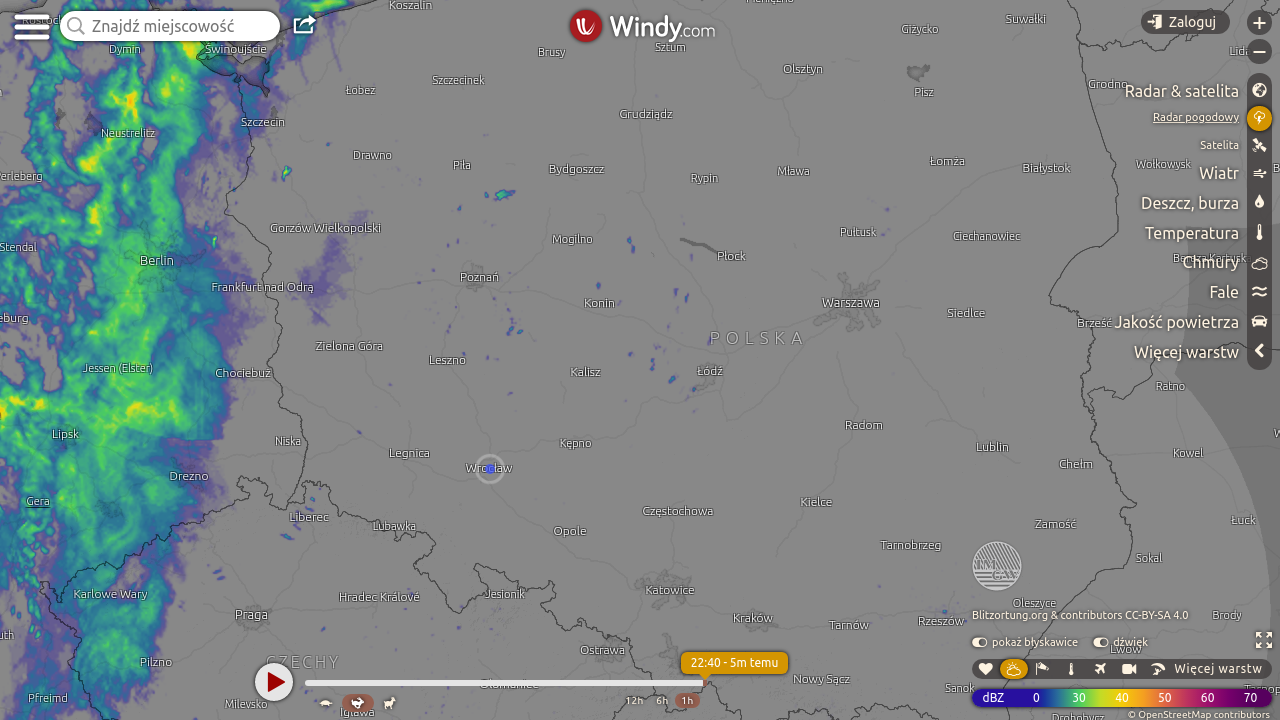
\includegraphics[width=\linewidth]{img/c1_windy.png}
    \caption{Widok wizualizacji dwuwymiarowej na stronie \textit{windy.com} wyświetlający informacje pogodowe na dwuwymiarowej mapie}
    \label{fig:c1_windy}
\end{figure}

Ważnym czynnikiem odbiorze wizualizacji, jest jej przystępność dla użytkownika. Profesjonalne, skomplikowane systemy nierzadko cechują się złożonym interfejsem użytkownika. Duża liczba opcji pomaga łatwo uzyskać pożądane dane przez doświadczonego użytkownika, ale odstraszyć może niezagłębionego w~temat odbiorcę. Przystępność odbioru wiąże się również z~szybkością uzyskania dostępu do samej platformy obsługującej wizualizację. Alternatywą dla instalowanych aplikacji desktopowych jest przeglądarka internetowa. Tworzy ona środowisko, które może być uruchomione na wielu systemach operacyjnych, również na urządzeniach mobilnych, a~zaimplementowane wspomaganie sprzętowe generowania grafiki i~interfejsy takie jak \textit{HTML5 Canvas}\cite{Canvas} i~\textit{WebGL}\cite{WebGL} czynią ją potężnym narzędziem do wydajnego wyświetlania złożonych grafik. 
Aplikacje webowe oczywiście nie będą nigdy dorównywać profesjonalnym aplikacjom dedykowanym konkretnej platformie, jednak stanowią ich dobrą i~ogólnodostępną alternatywę.

Innym kryterium definiującym wizualizację jest jej interaktywność. Definiuje ono w~jakim stopniu użytkownik może dostosować wyświetlany widok, zarządzać warstwami, sterować położeniem kamery, czy też wyszukiwać informacje. Dwuwymiarowy widok mapy (Rysunek \ref{fig:c1_windy}) pozwala jednoznacznie odnieść informacje z~różnych warstw do konkretnego miejsca na planecie. Z~kolej widok trójwymiarowy (Rysunek \ref{fig:c1_google_earth}) pozwala na obserwację sceny z~różnych perspektyw, pokazuje kulistość Ziemi i~redukuje efekty zniekształcenia danych związany z~techniką rzutowania sfery na płaszczyznę. Przy kamerze skierowanej prostopadle do płaszczyzny powierzchni, oraz w~bliskim powiększeniu widok taki jest porównywalny do widoku dwuwymiarowego. Czynniki te zdaniem autora pracy czynią taką wizualizację bardziej atrakcyjną dla ogólnego odbiorcy. Oczywiście wybór techniki wizualizacji zawsze zależy od konkretnego przypadku, jak i~od oczekiwanej wydajności, gdyż złożoność generowania grafiki w~przypadku wizualizacji trójwymiarowych jest z~reguły większa.


\begin{figure}[h]
    \centering
    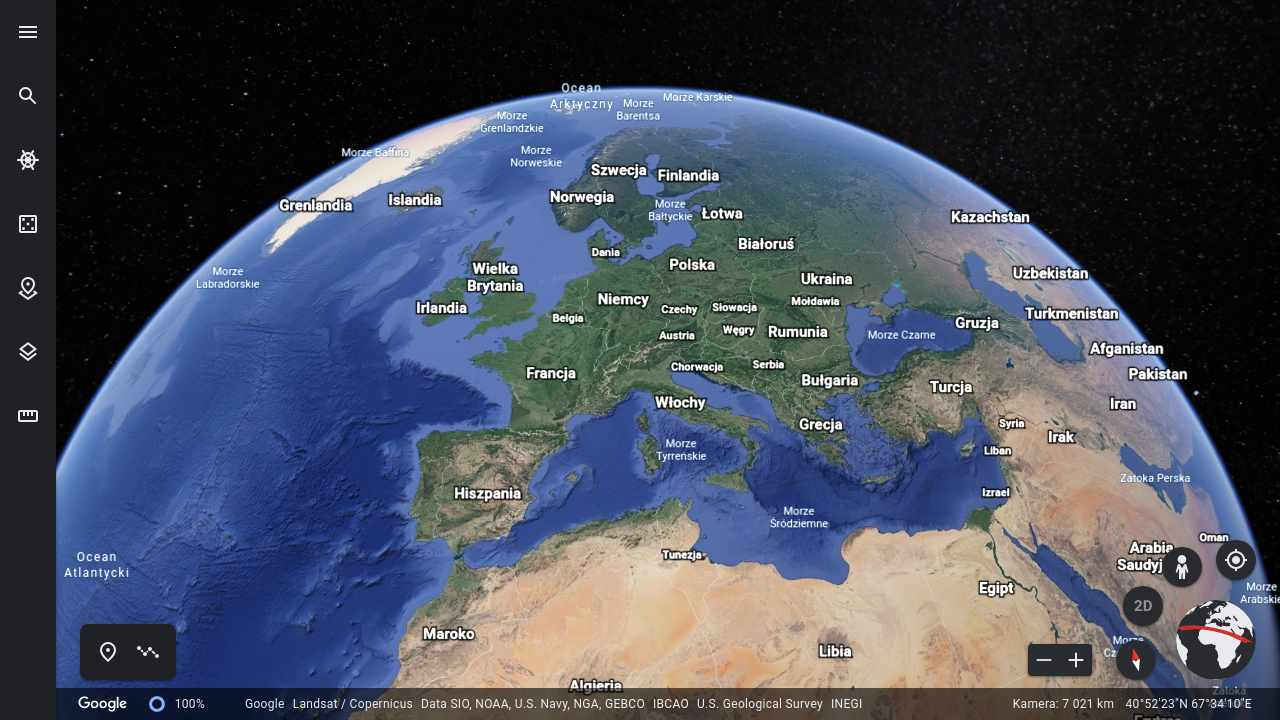
\includegraphics[width=\linewidth]{img/c1_google_earth.png}
    \caption{Widok wizualizacji trójwymiarowej na stronie \textit{earth.google.com}}
    \label{fig:c1_google_earth}
\end{figure}

\subsection{Podejścia do tworzenia wizualizacji}

Zadaniem twórcy wizualizacji jest zebranie i~przetworzenie danych na formę grafiki dwu lub trójwymiarowej. Od używanego systemu informacji przestrzennej zależy w~jaki sposób definiowana jest wizualizacja i~skutkiem tego, jaki poziom wiedzy i~umiejętności z~danej dziedziny jest potrzebny do jej stworzenia. System w~definicji wizualizacji opiera się na swoich założeniach. Aplikacje uruchamiane bezpośrednio w~środowisku systemu operacyjnego mogą być wyposażone w~rozbudowane kreatory i~edytory, które zaspokajają wymagania użytkowników. Pozwalają skupić się na zagadnieniach domenowych, na poprawności i~dokładności wizualizacji zamiast na aspektach generowania grafiki. 

W środowisku przeglądarki internetowej do tworzenia wizualizacji nie stosuje się zwykle rozbudowanych edytorów graficznych i~formularzy. Biblioteki wyświetlające dane geoprzestrzenne konfigurowalne są zwykle z~poziomu języka JavaScript. Przykładem takiej biblioteki jest \mbox{Cesium~\cite{CesiumJS}}. Potrafi ona generować wizualizacje dwu i~trójwymiarowej różnego rodzaju danych, a~jej konfiguracja następuje poprzez jej API, które dostarcza, ale też ogranicza jej możliwości (listing~\ref{lst:cesium}).

\begin{lstlisting}[label={lst:cesium}, language=javascript, caption={Konfiguracja podstawowej wizualizacji w~bibliotece Cesium. Żródło~\cite{CesiumJSExample}.}]
<script>
    Cesium.Ion.defaultAccessToken = 'your_access_token';
    var viewer = new Cesium.Viewer('cesiumContainer', {
        terrainProvider: Cesium.createWorldTerrain()
    });

    var tileset = viewer.scene.primitives.add(
        new Cesium.Cesium3DTileset({
            url: Cesium.IonResource.fromAssetId(your_asset_id)
        })
    );
    viewer.zoomTo(tileset);
</script>
\end{lstlisting}

Jeszcze innym podejściem, możliwym do zastosowania w~przypadku aplikacji i~desktopowych, i~webowych, jest dostarczenie twórcy tylko podstawowych abstrakcji (najczęściej interfejsów programistycznych) wizualizacji takich jak sterowanie kamerą, przekazywanie zdarzeń pochodzących od odbiorcy, czy interfejs służący do generowania obiektów na scenie dwu lub trójwymiarowej. Podejście daje to najwięcej możliwości, ale z~drugiej strony wymaga posiadania największej wiedzy o~funkcjonowaniu dostarczonych interfejsów.

W każdym wypadku istotnym czynnikiem ułatwiającym tworzenie wizualizacji jest dostarczona przez narzędzia i~biblioteki interaktywna dokumentacja. Powinna ona dobrze opisywać dostarczone rozwiązania ze strony praktycznej i~przez swoją interaktywność ułatwiać poruszanie się po niej użytkownikowi. 

\section{Cel projektu i~zawartość pracy}

Celem opisywanego projektu jest stworzenie biblioteki umożliwiającej definiowanie i~wyświetlanie trójwymiarowych wizualizacji w~środowisku przeglądarki internetowej. Projekt zakłada również stworzenie aplikacji webowej, która za pomocą osadzonej w~niej stworzonej biblioteki, umożliwia zarządzanie wyświetlaniem dostarczonych wizualizacji.

Rozdział drugi pracy opisuje szczegółowe wymagania postawione przed poszczególnymi komponentami aplikacji. Rozdział trzeci opisuje projekt i~implementację komponentu Silnika wyświetlającego wizualizację, a~rozdział czwarty przedstawia implementację przykładowych wizualizacji, które możliwe są do zdefiniowania korzystając z~interfejsów dostarczonych przez Silnik. W~rozdziale piątym opisana jest Aplikacja korzystająca z~komponentu Silnika zbierająca wizualizacje i~umożliwiająca filtrowanie i~przełączanie się pomiędzy nimi. Rozdział szósty opisuje sposoby testowania zaimplementowanych rozwiązań, a~rozdział siódmy przedstawia używane w~projekcie biblioteki pomocnicze wraz z~ich krótkim opisem. Rozdział ósmy podsumowuje całość projektu i~zwraca uwagę na problemy napotkane podczas implementacji, możliwości optymalizacji i~alternatywne rozwiązania poruszanych wcześniej kwestii projektowych i~implementacyjnych.
\chapter{Wymagania}

Ze względu na możliwy podział funkcjonalności projektu na wiele typów, zdefiniowano następujące pojęcia:
\begin{enumerate}
    \item Silnik - komponent odpowiedzialny za definicję i~wyświetlenie wizualizacji.
    \item Wizualizacja - konfigurowalny widok przedstawiający obiekty, których położenie zdefiniowano za pomocą współrzędnych geograficznych, na powierzchni sfery.
    \item Aplikacja - uruchomiona w~przeglądarce użytkownika strona umożliwiająca wybór i~wyświetlenie wizualizacji.
\end{enumerate} 

Silnik dostarcza komponenty i~interfejs programistyczny, dzięki którym można definiować, wyświetlać i~zarządzać wizualizacją.
Pozwala także na zdefiniowane wielu niezależnych wizualizacji. Z tego powodu można wyróżnić dwa typy użytkowników:

\begin{enumerate}
    \item Twórcę wizualizacji,
    \item Odbiorcę wizualizacji.
\end{enumerate}

Wymagania aplikacji zostały zdefiniowane z~podziałem na typ użytkownika.
Struktura danych definiująca renderowany obraz, zwana dalej będzie sceną.

\newcommand{\req}[3]{
    \stepcounter{#2}
    #1\_\arabic{#2} & #3 \\
    \hline
}

\section{Twórca wizualizacji}

\subsection{Wymagania funkcjonalne}

\newcounter{c_RA}

\begin{table}[H]
    \centering
    \begin{tabularx}{\textwidth}{|l|X|}
        \hline
        Numer & Wymaganie \\
        \hline
        \hline
        \req{RA}{c_RA}{Twórca może zdefiniować metadane wizualizacji określone przez interfejs Silnika.}
        \req{RA}{c_RA}{Twórca może zdefiniować statyczną scenę określając położenie obiektów na sferze z~wykorzystaniem długości i~szerokości geograficznej.}
        \req{RA}{c_RA}{Twórca do definicji sceny może wykorzystać interfejs tworzenia obiektów dostarczony przez aplikację lub załadować obiekty, materiały i~tekstury z~zewnętrznego źródła.}
        \req{RA}{c_RA}{Twórca może zagnieżdżać sceny predefiniowane w~silniku, oraz sceny wcześniej stworzonych przez siebie.}
        \req{RA}{c_RA}{Twórca może parametryzować sceny w~celu określonej ich modyfikacji w~procesie zagnieżdżania.}
        \req{RA}{c_RA}{Twórca może określić parametry początkowe obserwatora, dynamikę i~zakres jego ruchów:
            \begin{enumerate}
                \item położenie,
                \item prędkość i~przyspieszenie ruchu,
                \item ograniczenie przybliżenia,
                \item ograniczenie pozycji.
            \end{enumerate}
        }
        \req{RA}{c_RA}{Twórca może zdefiniować wygląd i~funkcjonalność panelu kontrolnego. Panel ten służyć będzie do zmiany parametrów wizualizacji i~obsługiwany będzie przez odbiorcę.}
        \req{RA}{c_RA}{Twórca, poprzez interfejs programistyczny dostarczony przez silnik, może aktualizować scenę w~dowolnym momencie, określonym przez siebie w~definicji wizualizacji.}
        \req{RA}{c_RA}{Twórca może definiować zachowania, które będą odpowiedzią na zdarzenia związane z~poruszaniem się po scenie generowane przez odbiorcę.}
    \end{tabularx}
    \caption{Wymagania funkcjonalne zdefiniowane dla twórcy wizualizacji }
    \label{tab:req_author_f}
\end{table}

\subsection{Wymagania niefunkcjonalne}

\begin{table}[H]
    \centering
    \begin{tabularx}{\textwidth}{|l|X|}
        \hline
        Numer & Wymaganie \\
        \hline
        \hline
        \req{RA}{c_RA}{Silnik powinien definiować i~w sposób jasny przekazywać potencjalnemu twórcy akceptowalną strukturę danych, plików i~katalogów, określającą jedną wizualizację.}
        \req{RA}{c_RA}{Włączenie zdefiniowanej wizualizacji do ich zbioru w~aplikacji powinno ustanowione być tylko w~jednym miejscu poprzez prosty interfejs.}
        \req{RA}{c_RA}{Dane wizualizacji muszą być ładowane asynchronicznie. Dane źródłowe definiujące scenę mogą być przetwarzane po stronie odbiorcy lub być przetworzone wcześniej i~pobrane.}
    \end{tabularx}
    \caption{Wymagania niefunkcjonalne zdefiniowane dla twórcy wizualizacji }
    \label{tab:req_author_nf}
\end{table}

\section{Odbiorca wizualizacji}
\newcounter{c_RU}

\subsection{Wymagania funkcjonalne}

\begin{table}[H]
    \centering
    \begin{tabularx}{\textwidth}{|l|X|}
        \hline
        Numer & Wymaganie \\
        \hline
        \hline
        \req{RU}{c_RU}{Odbiorca może zobaczyć dane dostępnych wizualizacji.}
        \req{RU}{c_RU}{Odbiorca może wyświetlić wybraną wizualizację.}
        \req{RU}{c_RU}{Odbiorca może poruszać się po wizualizacji, zmieniając położenia kamery, używając myszki lub klawiatury.}
        \req{RU}{c_RU}{Odbiorca może zobaczyć orientację kamery relatywnie do kierunku północnego i~ją zresetować.}
        \req{RU}{c_RU}{Odbiorca może wyświetlić lub ukryć panel sterujący wizualizacją dostarczony przez twórcę.}
    \end{tabularx}
    \caption{Wymagania funkcjonalne zdefiniowane dla odbiorcy wizualizacji }
    \label{tab:req_user_f}
\end{table}

\subsection{Wymagania niefunkcjonalne}

\begin{table}[H]
    \centering
    \begin{tabularx}{\textwidth}{|l|X|}
        \hline
        Numer & Wymaganie \\
        \hline
        \hline
        \req{RU}{c_RU}{Każda akcja użytkownika związana ze sterowaniem kamerą może zostać wykonana używając myszki lub równolegle klawiatury.}
       
    \end{tabularx}
    \caption{Wymagania funkcjonalne zdefiniowane dla odbiorcy wizualizacji }
    \label{tab:req_user_nf}
\end{table}

\section{Aplikacja}

\subsection{Wymagania niefunkcjonalne}

\begin{table}[H]
    \centering
    \begin{tabularx}{\textwidth}{|l|X|}
        \hline
        Numer & Wymaganie \\
        \hline
        \hline
        \req{RU}{c_RU}{Aplikacja powinna być stroną typu \textit{Single Page Application}.}
        \req{RU}{c_RU}{Jeśli to możliwe aplikacja powinna wykorzystywać sprzętową akcelerację obliczeń graficznych.}
        \req{RU}{c_RU}{Aplikacja powinna ustawiać i~obsługiwać adres URL w~przeglądarce definiujący wyświetlaną wizualizację.}
       
    \end{tabularx}
    \caption{Wymagania funkcjonalne zdefiniowane dla aplikacji }
    \label{tab:req_user_nf}
\end{table}




\chapter{Silnik}

Rozdział ten opisuje główny komponent tworzonego systemu nazwanego Silnikiem. Odpowiedzialny jest on za dostarczenie interfejsu definiowania trójwymiarowej wizualizacji i~jej późniejsze wyświetlanie. Narzuca również sposób pracy kamery i~umożliwia konfigurację jej parametrów.

Wszystkie obiekty wyświetlane na scenie, razem z~definicją ich wyglądu, tekstur i~dynamiki ruchów dostarcza wizualizacja. Jej obiekty mogą reagować na zdarzenia, które generuje użytkownik. Zainicjowanie procedury obsługi tych zdarzeń również komponent Silnika.

Najpierw w~sposób uproszczony opisany został sposób renderowania grafiki z~wykorzystaniem API WebGL oraz biblioteki Three.js. Następnie przedstawiono mechanizmy sterujące pracą kamery, a~następnie implementacja komponentu Silnika i~opisanych mechanizmów.

\section{WebGL i~ESSL}

WebGL jest dostępnym z~poziomu języka JavaScript API pozwalającym na renderowanie grafiki 3D w~przeglądarce. Złożone obiekty rysowane są tylko za pomocą punktów, linii i~trójkątów.  WebGL działa w~trybie \textit{immidiate}, który to wymusza na aplikacji wykonywanie bezpośrednio niskopoziomowych komend rysujących podstawowe obiekty 3D. Aplikacja korzystająca z~WebGL musi sama definiować abstrakcje podstawowych obiektów takich jak scena, kamera, czy światło. Podejście to jest bardzo elastyczne i~pozwala na optymalizację implementowanych rozwiązań w~zależności od potrzeb\cite[Rozdział 1]{RealTime3DGraphics}. WebGL korzysta z~akceleracji sprzętowej podczas renderowania grafiki - działa na GPU. W przypadku kart graficznych bez wsparcia dla ten technologii przeglądarki Google Chrome i~Internet Explorer 11 umożliwiają rysowanie z~użyciem CPU.

Drugim podejściem do renderowania grafiki jest podejście \textit{retained}, gdzie biblioteki z~niego korzystające implementują swoją abstrakcję sceny i~same zajmują się jej rysowaniem. Przykładem takiej biblioteki jest Windows Presentation Foundation\cite{WPF}.

Dostęp do API WebGL uzyskać można poprzez kontekst elementu \texttt{Canvas}. Na listingu \ref{lst:webglContext} pokazano pobranie kontekstu API WebGL do zmiennej \texttt{gl}. Wszystkie interakcje związane z~użyciem API będą odbywały się z~użyciem pobranego obiektu kontekstu. Numer w~identyfikatorze \texttt{’webgl2’} mówi, że używamy WebGL w~wersji drugiej.

\begin{lstlisting}[language=javascript, label={lst:webglContext}, caption={Pobranie kontekstu API WebGL do zmiennej}]
const canvas = document.getElementById('vis-container');
const gl = canvas.getContext('webgl2');
\end{lstlisting}

Obiekt kontekstu działa jak maszyna stanów. Przechowuje ustawiony stan do czasu jego zmiany przez aplikację. Wszystkie operacje renderowania grafiki korzystają z~globalnie ustawionych parametrów, które definiują stan kontekstu i~mają bezpośredni wpływ na efekt końcowy\cite[Rozdział 1]{RealTime3DGraphics}.

\subsubsection{Rysowanie sceny}

Rysowanie obiektu rozpoczyna się od utworzenia buforów danych i~umieszczenia w~nich współrzędnych wierzchołków oraz kolejności, według której wierzchołki mają brać udział w~procesie rysowania. Kolejność ma istotne znaczenie w~przypadku różnych trybów rysowania oraz, Cullingu czyli określania widocznej strony rysowanego trójkąta. Bufory są reprezentowane zewnętrznie jako tablice \texttt{TypedArray}. Przechowują one jedynie surowe dane w~postaci binarnej \cite{TypedArrays}. W języku JavaScript występuje jeden typ \texttt{number} przechowujący liczby, które wewnętrznie reprezentowane są jako 64b liczba zmiennoprzecinkowa. Dodatkowo każda zmienna numeryczna jest obiektem typu \texttt{Number} z~własnymi metodami. Użycie buforów z~interfejsem tablicy przyspiesza operacje na danych.

\subsubsection{Shadery}

W WebGL'u \textit{programem} nazywane są skompilowane przez kontekst shadery. Są to krótkie programy napisane w~specjalistycznym języku, którym w~przypadku WebGL'a jest ESSL(ang. OpenGL ES Shading Language). Przypomina on składnią język C/C++\cite{ESSL} i~zawiera wbudowane funkcje wymagane do operacji matematycznych takich jak iloczyn skalarny wektorów, czy mnożenie macierzy. Na wspomniany \textit{program} składają się dwa shadery - \texttt{vertex shader} i~\texttt{fragment shader}. \texttt{Vertex shader}, uruchamiany jako pierwszy, pobiera dane o~wierzchołkach z~buforów, oraz korzystając ze stałych (\texttt{uniforms}) oblicza finalną pozycję wierzchołka. W większości przypadków shader ten odpowiada również za obliczenie innych parametrów wierzchołka takich jak kolor, jego wektor normalny, czy też współrzędne tekstur. Dla każdego wierzchołka wyliczone wartości wysyłane są dalej do shadera \texttt{fragment shader}.

\texttt{Fragment shader} odpowiada za wyliczenie koloru pojedynczego pixela. Dale wysłane z~\texttt{vertex shader}'a w~zmiennych typu \texttt{varying} są automatycznie interpolowane dla każdego punktu w~renderowanym trójkącie na podstawie trzech wierzchołków.

W shaderach, po dostarczeniu odpowiednich danych, realizowane są abstrakcje takie jak kamera, oświetlenie, czy materiały.

\subsubsection{Obliczanie finalnej pozycji wierzchołków}

W grafice 3D każdy model reprezentowany jest przez zbiór punktów i~informacji o~kolejności ich rysowania. Model może mieć swoją pozycję w~świecie 3D, a~obserwator może znajdować się w~różnych miejscach sceny. WebGL sam w~sobie nie posiada abstrakcji kamery i~do wyświetlenia sceny z~konkretnej perspektywy konieczne jest przemieszczenie wszystkich wierzchołków geometrii. Transformacja pozycji wierzchołków odbywa się za pomocą przekształceń afinicznych, które transformują pozycję zbioru wierzchołków i~nie zaburzają relacji pomiędzy nimi. Efektywnie transformacja taka jest mnożeniem macierzy transformacji o~wymiarach 4x4 i~wektora z~dodaną czwartą współrzędną równą 1, co daje nowy wektor współrzędnych wierzchołka.

Przekształcenia związane z~pozycją modelu i~kamery w~świecie wyrażane są za pomocą macierzy. Macierzowy opis przekształceń możliwy jest dzięki zastosowaniu współrzędnych jednorodnych\cite{Homogeneous}. Transformacja pozycji modelu odbywa się z~pomocą macierzy $M$, a~transformacja pozycji związana z~położeniem kamery z~pomocą macierzy widoku $V$. Wyliczanie współrzędnych wierzchołka w~układzie współrzędnych świata pokazano w~równaniu \ref{eq:MV}.

Aby uzyskać wyjściową pozycję piksela na ekranie konieczne jest pomnożenie macierzy projekcji i~wektora pozycji wierzchołka w~układzie współrzędnych świata (równanie \ref{eq:MVP}). Macierz projekcji odpowiada za transformację współrzędnych wierzchołka do sześcianu o~wymiarach 2x2x2 i~środku w~punkcie $(0, 0, 0)$. Transformacja ta może być perspektywiczna, gdzie przekształceniu ulega przestrzeń w~kształcie ostrosłupa ściętego. Może być też ortograficzna, gdzie przekształceniu ulega przestrzeń w~kształcie prostopadłościanu. Punkty leżące poza tą przestrzenią nie są rysowane. Współrzędne $(x, y)$ transformowanych wierzchołków są współrzędnymi \textit{NDC} (ang. Normalized Device Coordinates), niezależnymi od urządzenia. Dzięki temu mogą być one łatwo przekształcone na piksele elementu Canvas, gdzie punkt $(0, 0)$ znajduje się w~lewem górnym rogu. Podejście to uniezależnia generowanie pikseli od elementu wyświetlającego, do którego trzeba dostosować tylko sposób przekształcenia współrzędnych \textit{NDC}.

\begin{equation}
    \label{eq:MV}
    p' = VM \cdot \begin{bmatrix}
        p_{1} \\
        p_{2} \\
        p_{3} \\ 
        1
      \end{bmatrix}
\end{equation}
\begin{eqexpl}[25mm]
    \item{$M$} macierz transformacji pozycji modelu
    \item{$V$} macierz transformacji widoku
    \item{$p'$} wektor pozycji wierzchołka w~układzie współrzędnych widoku
    \item{$p$} wektor pozycji modelu w~układzie współrzędnych świata
\end{eqexpl}

\begin{equation}
\label{eq:MVP}
    v = P \cdot \begin{bmatrix}
        p'_{1} \\
        p'_{2} \\
        p'_{3} \\ 
        1
      \end{bmatrix}
\end{equation}
\begin{eqexpl}[25mm]
    \item{$P$} macierz projekcji
    \item{$p'$} wektor pozycji wierzchołka w~układzie współrzędnych widoku
\end{eqexpl}
\vspace{\baselineskip}
Kalkulacja pozycji modeli oraz kamery ma szczególne znaczenie przy złożonym zachowaniu kamery oraz sceny w~komponencie Silnika.

\subsection{Three.js}

Three.js\cite{threejs} jest biblioteką 3D, która domyślnie do renderowania grafiki używa WebGL. Ułatwia ona rozpoczęcie pracy z~grafiką 3D i~jednocześnie nie nakłada ograniczeń związanych z~niskopoziomową konfiguracją wyświetlanej sceny. Pozwala ona na opisanie sceny, obiektów, świateł i~materiałów w~postaci obiektowej. Posiada rozbudowany system animacji oraz wsparcie dla systemów wirtualnej rzeczywistości. Na listingu \ref{lst:threejs:base} pokazano kod aplikacji, która wyświetla zielony sześcian.

\begin{lstlisting}[language=javascript, label={lst:threejs:base}, caption={Hello World w~świecie grafiki 3D}]
    const scene = new THREE.Scene();
    const camera = new THREE.PerspectiveCamera( 75, window.innerWidth / window.innerHeight, 0.1, 1000 );
    
    const renderer = new THREE.WebGLRenderer();
    renderer.setSize( window.innerWidth, window.innerHeight );
    document.body.appendChild( renderer.domElement );

    const geometry = new THREE.BoxGeometry();
    const material = new THREE.MeshBasicMaterial( { color: 0x00ff00 } );
    const cube = new THREE.Mesh( geometry, material );
    scene.add( cube );

    camera.position.z = 5;

    function animate() {
        requestAnimationFrame( animate );
        renderer.render( scene, camera );
    }
    animate();
\end{lstlisting}

Na początku tworzony jest obiekt sceny, która jest kontenerem na pozostałe wyświetlane obiekty oraz światła. Następnie tworzony jest obiekt kamery, który definiuje właściwości, w~tym wypadku, projekcji perspektywicznej. Utworzony dalej obiekt \texttt{THREE.WegGLRenderer} odpowiedzialny jest za utworzenie i~przechowywanie referencji do obiektu \texttt{Canvas}, na którym, w~głównej pętli programu, rysuje dostarczoną scenę z~perspektywy wybranej kamery. Odpowiada za to wywołanie \texttt{renderer.render(scene, camera)}.

Geometrię kostki definiuje obiekt \texttt{THREE.BoxGeometry}, która z~domyślnymi argumentami konstruktora jest sześcianem o~wymiarach 1x1x1. Obiekt ten posiada atrybuty ułatwiające zarządzanie wygenerowaną geometrią. Zwykłe obiekty geometrii są konwertowane do typu \texttt{BufferGeometry} w~procesie renderowania, Wtedy dane wierzchołków są umieszczane w~buforach, które mogą być bezpośrednio wykorzystane w~interakcji z~WebGL'em. Three.js pozwala tworzyć geometrię w~sposób bardziej efektywny, jednak gorzej zarządzalny, wykorzystując klasy pochodne klasy \texttt{BufferGeometry}, takie jak \texttt{BoxBufferGeometry}.

Elementy wyglądu rysowanych geometrii określa materiał. W Three.js obiektami je reprezentujące są pochodne klasy \texttt{Material}. Umożliwiają ustawienie koloru, tekstur, różnego rodzaju map, a~w przypadku światła parametry jego interakcji z~powierzchnią obiektu. W procesie rysowania obiektu, atrybuty jego materiału, oraz atrybuty obiektów ważnych dla wyglądu rysowanego obiektu, na przykład świateł, są wysyłane do shaderów w~postaci stałych (\texttt{uniforms}). Sam materiał definiuje jednoznacznie działanie shaderów, wykorzystanych w~procesie jego rysowania. Przykład shadera dla materiału \texttt{MeshBasicMaterial} pokazano na listingu \ref{lst:matVert}.

\begin{lstlisting}[language=C++, label={lst:matVert}, caption={
    Fragmenty vertex shadera materiału \texttt{MeshBasicMaterial}}
]
#include <common>
/* ... */

void main() {
    /* ... */
	#include <color_vertex>
    /* ... */

	#include <begin_vertex>
	/* ... */
	#include <project_vertex>
	/* ... */
}
\end{lstlisting}

Shadery różnych materiałów współdzielą pomiędzy sobą wiele swoich części. Dlatego zastosowano dyrektywę \texttt{\#include} w~celu umieszczenia w~kodzie wspólnych części. Na listingu \ref{lst:vertProject}, w~części \texttt{project\_vertex}, widać właściwy proces obliczania pozycji wierzchołka przedstawiony na równaniach \ref{eq:MV} i~\ref{eq:MVP}. Macierz projekcji mnożona jest przez połączoną macierz modelu i~widoku oraz zmienną wektorową \texttt{mvPosition}. Wynikowy wektor wpisywany jest do specjalnej zmiennej globalnej \texttt{gl\_Position}, której zawartość informuje resztę składowych procesu generowania grafiki o~wyniku kalkulacji. 

\begin{lstlisting}[language=C++, label={lst:vertProject}, caption={
    Fragmenty części \texttt{project\_vertex} vertex shadera}
]
vec4 mvPosition = vec4( transformed, 1.0 );
/* ... */
mvPosition = modelViewMatrix * mvPosition;
gl_Position = projectionMatrix * mvPosition;
\end{lstlisting}

Three.js dostarcza również wiele narzędzi ułatwiających operacje matematyczne na wektorach oraz macierzach. Pozwala między innymi na interpolację liniową i~sferyczną wektorów, generowanie macierzy transformacji, czy reprezentowanie obrotów za pomocą kątów Eulera lub kwaternionów.

\section{Praca kamery}

Komponent Silnika wyświetla scenę, w~której kamera orbituje wokół jednego punktu. Dodatkowo użytkownik może zmienić orientację kamery względem punktu na powierzchni sfery. Opis pracy kamery odnosić się będzie do obiektu sfery i~jej powierzchni, jednak nic nie stoi na przeszkodzie, aby kamera orbitowała wokół innego obiektu. W tym podrozdziale opis mechanizmów jest przedstawiony w~oderwaniu od ich implementacji w~projekcie. Finalnie, pozycję kamery relatywnie do środka sfery opisują dwie orbity. Orbitą, w~kontekście pracy kamery, nazwana została para wektorów określająca obrót od wektora odniesienia i~odległość od punktu jego zaczepienia.

Wspomniane orbity nazwano orbitą lokalną i~orbitą globalną. Orbita globalna odpowiedzialna jest za pozycję kamery nad punktem obiektu sfery. Orbita lokalna określa orientacją kamery względem punktu, nad którym się znajduje. Taki podział sceny wprowadza również dwa układy odniesienia.

\begin{enumerate}
    \item Układ obserwatora - układ, w~którym znajduje się obserwator i~wszystkie obiekty są pozycjonowane relatywnie do obiektu kamery. Jest to domyślny układ renderowanej sceny.
    \item Układ wizualizacji - układ, w~którym obiekty pozycjonowane są relatywnie do mogącej obracać się sfery. Obiekty umieszczane są w~obracającej się grupie.
\end{enumerate}

Żeby przybliżyć zależności pomiędzy tymi układami, można posłużyć się przykładem. Aby symulować cykl dnia i~nocy, światło musi być pozycjonowane w~układzie wizualizacji, ponieważ jest niezależne od ruchu kamery. Aby światło oświetlało zawsze widoczną stronę planety, musi być ono pozycjonowane w~układzie obserwatora. Ogólny graf sceny przedstawiono na diagramie \ref{fig:c3_scene_graph}.

\begin{figure}[h]
    \centering
    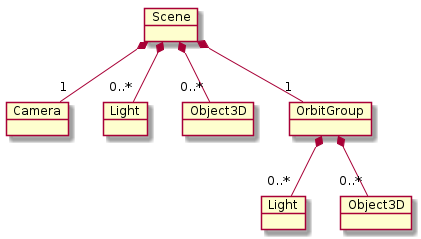
\includegraphics[height=5.5cm]{diagrams/out/c3_scene_graph.png}
    \caption{Ogólny graf sceny wizualizacji}
    \label{fig:c3_scene_graph}
\end{figure}

\subsection{Orbita globalna}

Orbitę globalną definiują dwa wektory - $g_v$ i $g_{up}$ na rysunku \ref{fig:orbits}. Pierwszy rozciągnięty jest od środka sfery do punktu, wokół którego orbituje kamera. Drugi jest wektorem jednostkowym do niego prostopadłym określającym orientację sfery w osi pierwszego wektora. W późniejszym opisie działanie \textit{na orbicie}, na przykład obrót orbity, oznacza wykonanie tej samej transformacji na obu wektorach. W ten sposób oba wektory nigdy nie zmienią swojej wzajemnej orientacji.

Użytkownik za pomocą myszy lub klawiatury może obrócić sferę, a konkretnie grupę obrotu (\texttt{OrbitGroup} na diagramie \ref{fig:c3_scene_graph}) i zawierane przez nie obiekty. Jest to efektywnie zmianą punktu, nad którym znajduje się kamera, pomimo tego, że jej pozycja się nie zmienia. Jako, że obrót sfery definiowany jest abstrakcję orbity, cała operacja sprowadza się do jej odpowiedniego obrócenia. 

Parametrami specyficznymi dla orbity globalnej są:
\begin{enumerate}
    \item tryb pracy orbity - określa czy podczas przesuwania orbity ma ona zachowywać swoją orientację w kierunku północnym. Wydzielono tryb \textit{swobodny} i \textit{kompas}.
\end{enumerate}

\subsection{Orbita lokalna}

Orbitę lokalną, podobnie jak globalną, definiują dwa wektory - $l_v$ i $l_{up}$ na rysunku \ref{fig:orbits}. Pierwszy rozciągnięty jest od punktu, wokół którego orbituje kamera, do kamery. Drugi jest wektorem jednostkowym do niego prostopadłym określającym orientację kamery w osi pierwszego wektora.

Użytkownik za pomocą myszy lub klawiatury może zmienić punkt orbitowania kamery. Jest to efektywnie zmianą położenia kamery w układzie obserwatora. Jako, że pozycja kamery definiowany jest przez abstrakcję orbity, cała operacja sprowadza się do jej odpowiedniego obrócenia.

Pierwszy wektor orbity lokalnej może mieć zmienną długość. Reprezentuje ona odległość obserwatora do punktu na powierzchni sfery. 

Parametrami specyficznymi dla orbity lokalnej są:
\begin{enumerate}
    \item współczynnik przybliżenia - jak powinna zmienić się odległość kamery od punktu na powierzchni sfery podczas jednej akcji przybliżenia.
    \item granice przybliżenia - minimalna i maksymalna odległość kamery od punktu na powierzchni sfery.
\end{enumerate}

\subsection{Parametry wspólne dla obu orbit}

Dla obu orbit wyróżniono wspólne parametry. Są nimi:
\begin{enumerate}
    \item granice - wyrażony w radianach zakres współrzędnych geograficznych definiujący fragment sfery, nad którym kamera może się znaleźć. Może służyć na przykład do ograniczenia obszaru poruszania się użytkownika tylko do jednej półkuli lub jednego miasta.
    \item prędkość obrotu - współczynnik sterujący prędkością obrotu danej orbity.
\end{enumerate}

Wszystkie parametry, ogólne i te specyficzne dla każdej z orbit mogą być konfigurowane przez wizualizację.

\begin{figure}[]
    \centering
    \newlength{\gRadius}
\setlength{\gRadius}{3cm}
\newlength{\lRadius}
\setlength{\lRadius}{4cm}
\tikzset{>={Latex[scale=1.5]}}

\begin{tikzpicture}[scale=1.25]
    \coordinate (G) at (90:\gRadius);
    \coordinate (G_up) at ($(G) +(0:1)$);
    \coordinate (L) at ($(G) +(135:2)$);
    \coordinate (L_up) at ($(L) +(45:1)$);
    \coordinate (center) at (90:0);


    \begin{scope}
      \clip (-\gRadius,0) rectangle (\gRadius,\gRadius);
      \draw[thick] circle (\gRadius);
  \end{scope}

    \draw[->] (center) -- (G) node[midway,left] {$\vec g_v$};
    \draw[->] (G) -- (G_up) node[midway,above] {$\vec g_{up}$};
    \draw[fill] (G) circle (1.5pt) node[above] {$c_g$};
   
    \draw[->] (G) -- (L) node[midway,above] {$\vec l_v$};
    \draw[->] (L) -- (L_up) node[midway,above] {$\vec l_{up}$};
    \draw[fill] (L) circle (1.5pt) node[above] {$c_l$};


\end{tikzpicture}


    \caption{Schemat orbit w specyficznym przypadku dwóch wymiarów}
    \label{fig:orbits}
\end{figure}



\subsection{Obrót orbity globalnej}

Algorytm obrotu orbity globalnej wykonywany jest dla każdego zdarzenia przesunięcia myszy użytkownika podczas gestu chwycenia, przeciągnięcia i upuszczenia wygenerowanym przez element \texttt{Canvas}. Obrót wymaga obliczenia jego chwilowej osi i kąta.

\subsubsection{Kwaterniony}
%TODO:Opisać

%TODO: wyliczanie osi i kąta obrotu + korekcja + korekcja trybu

\subsection{Obrót orbity lokalnej}

\subsection{Animacje - płynność ruchów}

\section{Implementacja}

\chapter{Wizualizacje}

Rozdział ten opisuje obiekty wizualizacji, które powstały podczas rozwoju komponentu Silnika. Ich opis będzie postępował w~kolejności od najprostszych, do tych bardziej skomplikowanych, których te prostsze stanową podstawę. Opisane zostaną również bardziej złożone aspekty renderowania grafiki, jeśli wizualizacje z~takich korzystają.
Wizualizacje te są po części demonstracją możliwości Silnika i~nie były tworzone z~zachowaniem stuprocentowej dokładności odwzorowania zjawisk.

\section{Gwiazdy}

Wizualizacja ta wyświetla teksturę kosmosu nałożoną na wewnętrzną część sfery - rysunek~\ref{fig:c4_starsVis}. Kamera znajduje się w~jej środku, więc przeciągnięcie widoku w~jedną stronę skutkuje przesunięciem się tekstury kosmosu w~przeciwną. Wizualizacja ta nie modyfikuje ustawień kamery oraz nie definiuje swojego panelu kontrolnego. Tekstura gwiazd pochodzi ze strony \url{https://www.solarsystemscope.com/}~\cite{SolarTextures}. 

\begin{figure}[h]
  \centering
  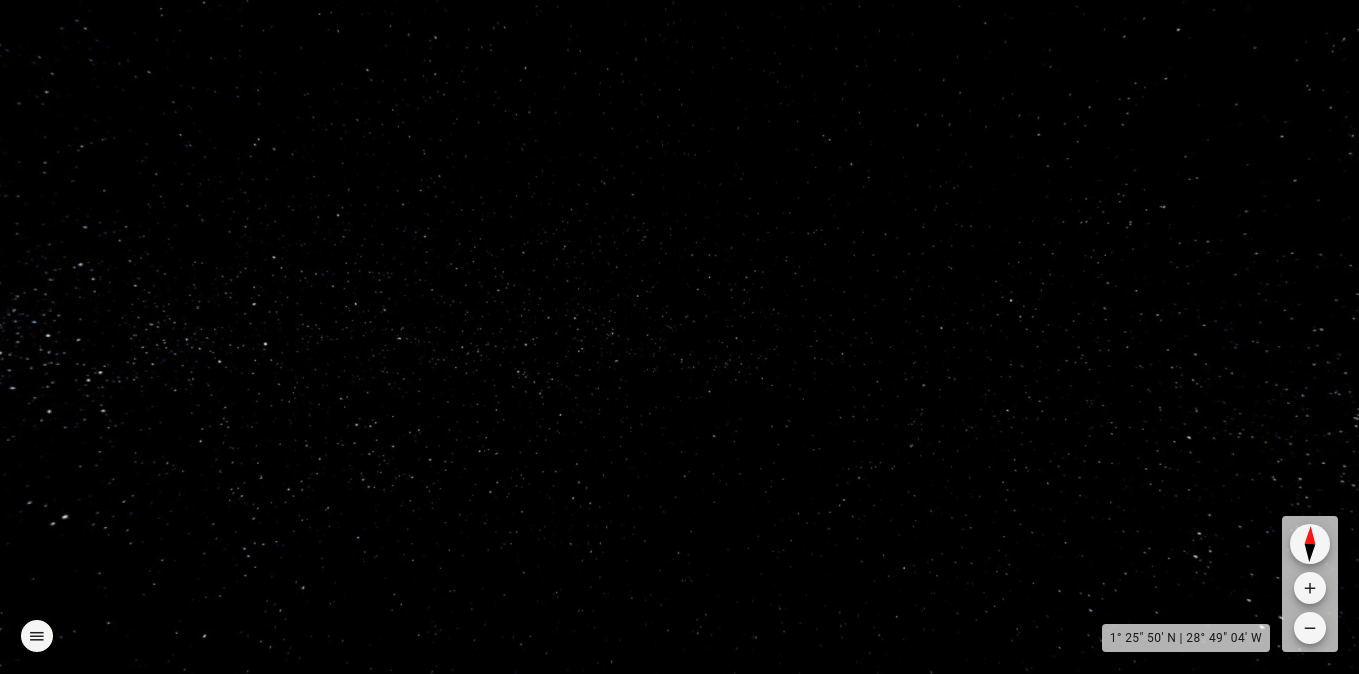
\includegraphics[width=\linewidth]{img/c4_starsVis.png}
  \caption{Wizualizacja gwiazd - klasa \texttt{StarsVis}}
  \label{fig:c4_starsVis} 
\end{figure}

Na listingu~\ref{lst:starsVis} pokazano część klasy \texttt{StarsVis} definiującą tę wizualizację. Sfera tworzona jest z~użyciem klasy \texttt{THREE.SphereGeometry}, a~jej materiał \texttt{THREE.MeshBasicMaterial} zawiera ustawienia definiujące jej wyświetlanie. Ustawienie \mbox{\texttt{side:THREE.BackSide}} sprawia, że teksturowane są odwrotna niż zwykle strona rysowanego trójkąta. Ustawienia \mbox{\texttt{depthWrite:false}} oraz \mbox{\texttt{depthFunc:THREE.NeverDepth}} sprawiają, że obiekt nie będzie wpływał na wartość z-bufora, oraz będzie rysowany zawsze za innymi obiektami, co jest oczekiwane od obiektu tła. 


\begin{lstlisting}[float, language=javascript, label={lst:starsVis}, caption={
  Fragmenty klasy \texttt{StarsVis}}
]
/* ... */
export default class StarsVis extends Visualization {
private stars = new THREE.SphereGeometry(40000, 10, 10);
private starsMaterial = new THREE.MeshBasicMaterial({
  side: THREE.BackSide,
  map: new THREE.TextureLoader().load(starsMap),
  depthWrite: false,
  depthFunc: THREE.NeverDepth,
});
private mesh = new THREE.Mesh(this.stars, this.starsMaterial);
/* ... */
public setupCamera(camera: TrackballCamera): void {
  //
}
public setupScene(scene: THREE.Scene, group: THREE.Group): void {
  this.mesh.renderOrder = 0;
  group.add(this.mesh);
}
public update(deltaFactor: number): void {
  this.mesh.rotation.y = TimeService.getHourAngle();
}
/* ... */
}
\end{lstlisting}

Obiekt 3D \texttt{THREE.Mesh} w~metodzie \texttt{update} obracany jest w~osi $OY$ o~pewien kąt. Kąt ten wynika z~czasu słonecznego, ponieważ wizualizacja ta domyślnie ma stanowić tło dla wizualizacji Ziemi w~czasie rzeczywistym. Może być ona również rozszerzona, aby obsługiwać każdy inny dowolny czas. Kiedy kamera jest nieruchowa względem punktu na Ziemi, jej obrót w~okół własnej osi widoczny jest jako obrót tła w~przeciwnym kierunku. Klasa TimeService, dokładniej opisana w~dalszej części pracy, zawiera metodę \texttt{getHourAngle}, która dla danej strefy czasowej oblicza kąt obrotu Słońca od danej długości geograficznej o~danym czasie~\cite{SolarTime}. Punktem odniesienia jest południk $\ang{0}$ i~strefa czasowa \textit{+00:00}. 

\section{Atmosfera}

Wizualizacja atmosfery stanowi wizualną dekorację dla innych wizualizacji. Składa się ona z~dwóch osobno generowanych części. Wizualnie atmosfera to poświata widoczna nad powierzchnią planety, która zanika wraz ze wzrostem wysokości punktu nad powierzchnią. Na efekt też wpływa sama grubość atmosfery, jej skład chemiczny, oraz gęstość w~poszczególnych jej partiach.

Utworzona wizualizacja nie posiada rozbudowanych możliwości konfiguracji i~została stworzona do współpracy z~wizualizacją Ziemi w~dużej skali. Na efekt poświaty składają się dwa obiekty. Pierwszym jest sfera, której średnica odpowiada średnicy planety razem z~grubością atmosfery. Wyświetlana jest jej wewnętrzna część i~znając pozycje obserwatora, wyświetlana jest właściwie zanikająca poświata. Drugim obiektem jest sfera rozmiarów planety, która zawsze generowana jest przed nią i~odpowiada za poświatę widoczną bezpośrednio nad planetą. Na rysunku~\ref{fig:c4_atmosphereVis} przedstawiono efekt atmosfery bez planety. Istotne są tutaj jedynie krawędzie widocznego okręgu, ponieważ jego środek ukryty będzie za planetą. Na rysunku~\ref{fig:atmosphere} przedstawiono schemat elementów kluczowych dla wyliczenia parametrów atmosfery. Kamera znajduje się w~punkcie $c_l$. Okrąg rysowany linią ciągłą symbolizuje powierzchnię planety, a~linią przerywaną, zasięg atmosfery. Wektor $\vv t$ stanowi przedłużenie wektora $\vv{g_v}$ o~grubość atmosfery. Widoczny dla obserwatora fragment atmosfery jest łukiem pomiędzy punktami $c_{gtb}$~i~$c_{gt}$.

\begin{figure}
\centering
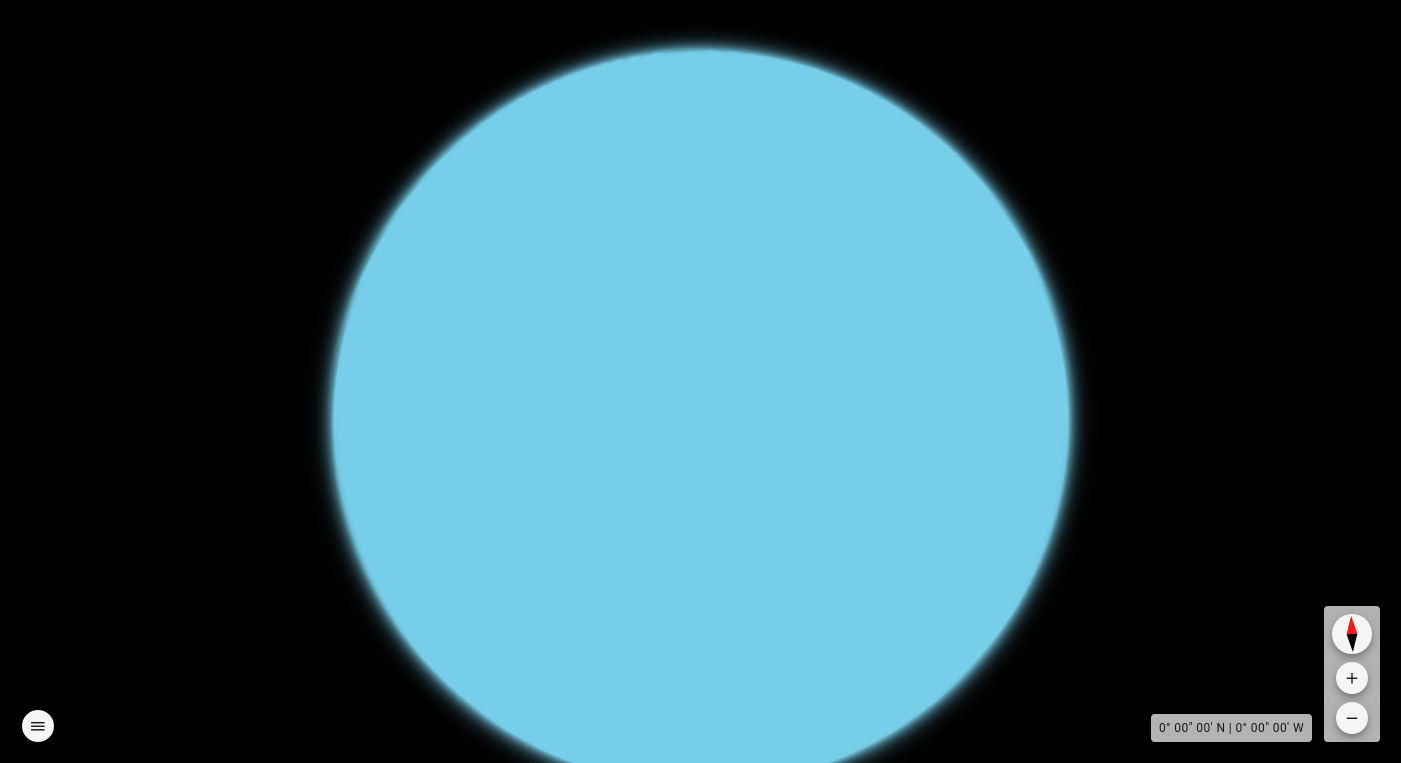
\includegraphics[width=\linewidth]{img/c4_atmosphereVis.png}
\caption{Wizualizacja atmosfery - klasa \texttt{AtmosphereVis}}
\label{fig:c4_atmosphereVis} 
\end{figure}

\begin{figure}[h]
\centering
\newlength{\gRadius}
\setlength{\gRadius}{3cm}
\newlength{\atmThickness}
\setlength{\atmThickness}{1cm}
\begin{tikzpicture}[scale=1.5]

    \coordinate (G) at (65:\gRadius);
    \coordinate (GT) at (65:\gRadius+\atmThickness);
    \coordinate (camera) at (90:\gRadius + \atmThickness + 1cm);
    \coordinate (center) at (90:0);
    \coordinate (atmTangent) at (126.869897646:\gRadius + \atmThickness);
    \coordinate (gTangent) at (143.130102354:\gRadius);
    \coordinate (atmBackTangent) at (184.539722109:\gRadius + \atmThickness);

    \draw[thick] circle (\gRadius);
    \draw[thick,dashed] circle (\gRadius+\atmThickness);
    \draw[red, fill=red] (0,5cm) circle (5pt);
    \draw[->] (center) -- (camera) node[midway,above,sloped] {\tiny$\vec G + \vec L$};
    \draw[->] (center) -- (G) node[midway,above,sloped] {\tiny$\vec G$};
    \draw[->] (G) -- (GT) node[midway,above,sloped] {\tiny$\vec T$};
    \draw[->] (G) -- (camera) node[midway,above,sloped] {\tiny$\vec L$};
    \draw[dashed] (camera) -- (atmTangent);
    \draw[dashed] (camera) -- (gTangent);

    \draw[->] (center) -- (atmTangent) node[midway,below,sloped] {\tiny$\vec G + \vec T$ };
    \draw pic["$\alpha$",draw=blue,thick,blue, ->, angle eccentricity=1.2, angle radius = 1.3cm]  {angle=camera--center--atmTangent};
    \draw pic["$\cdot$",draw, -, angle eccentricity=0.5, angle radius = 0.4cm]  {angle=center--atmTangent--camera};

    \draw[->] (center) -- (gTangent) node[midway,below,sloped] {\tiny$\vec G$ };
    \draw pic["$\beta$",draw=orange,thick,orange, ->, angle eccentricity=1.2, angle radius = 1.8cm]  {angle=camera--center--gTangent};
    \draw pic["$\cdot$",draw, -, angle eccentricity=0.5, angle radius = 0.4cm]  {angle=center--gTangent--camera};

    \draw[dashed] (gTangent) -- (atmBackTangent);
    \draw pic["$\cdot$",draw, -, angle eccentricity=0.5, angle radius = 0.4cm]  {angle=atmBackTangent--gTangent--center};
    \draw pic["$\gamma$",draw=red,thick,red, ->, angle eccentricity=1.2, angle radius = 1cm]  {angle=gTangent--center--atmBackTangent};
    \draw[->] (center) -- (atmBackTangent) node[midway,below,sloped] {\tiny$\vec G + \vec T$ };

\end{tikzpicture}


\caption{Schemat elementów kluczowych dla wyliczenia parametrów atmosfery}
\label{fig:atmosphere}
\end{figure}

\begin{lstlisting}[float, language=javascript, label={lst:atmosphereVis}, caption={
Fragmenty klasy \texttt{StarsVis}}
]
public atmosphereMaterial = new THREE.ShaderMaterial({
vertexShader: vertexShader,
fragmentShader: fragmentShader,
uniforms: {
  start: { value: 1 },
  stop: { value: 0.6 },
  fadeOut: { value: 0 },
  light: { value: 0 },
  power: { value: 1.25 },
  glowColor: { value: new THREE.Color(0x87ceeb) },
  viewVector: { value: new THREE.Vector3() },
  ...THREE.UniformsLib.lights,
},
depthFunc: THREE.NeverDepth,
lights: true,
transparent: true,
side: THREE.BackSide,
depthWrite: false,
});
\end{lstlisting}

Na listingu~\ref{lst:atmosphereVis} przedstawiono inicjalizację materiału odpowiedzialnego za poświatę nad planetą. Klasa \texttt{THREE.ShaderMaterial} pozwala kontrolować cały proces rysowania punktów, ponieważ wymaga dostarczenia obydwu typów shaderów. Tak jak w~przypadku materiału w~wizualizacji \texttt{StarsVis}, materiał definiuje też ustawienia modyfikacji z-bufora i~strony wyświetlanego trójkąta. Materiał definiuje również stałe dla jednego procesu rysowania (\texttt{uniforms}). Stałe te są aktualizowane w~każdym cyklu animacji. 
W procesie rysowania poświata generowana jest w~zależności od kąta pomiędzy wektorem normalnym płaszczyzny dla wierzchołka, a~wektorem określającym kierunek obserwacji. Niżej opisano stałe przekazywane do materiału.

\subsubsection{Uniform \texttt{start}}
Uniform \texttt{start} to ułamek liczby $\pi$ w~zakresie $\lbrack0; 1\rbrack$, który stanowi kąt wektora obserwatora z~wektorem normalnym wierzchołka, od którego rozpoczyna się rysowanie poświaty. Wartość ta zawsze wynosi $1$, co oznacza, że poświata rysowana jest od wierzchołków najdalej od kamery. Jego wektor normalny na rysunku \ref{fig:atmosphere} oznaczony został symbolem $\vv n$. Kąt między nim, a~wektorem $\vv{g_v} + \vv{l_v}$ wynosi $\ang{180}$, czyli $1 \cdot \pi$.

\subsubsection{Uniform \texttt{stop}}
Uniform \texttt{stop} to ułamek liczby $\pi$ w~zakresie $\lbrack0; 1\rbrack$, który stanowi kąt wektora obserwatora z~wektorem normalnym wierzchołka, od którego kończy się rysowanie poświaty o~pełnej przezroczystości. Ostatnim widocznym z~kamery punktem jest punkt $c_{gtb}$. Dalsza część schowana jest za planetą. Kąt ten wyliczany jest z~zależności $\beta+\gamma$. Sposób wyliczenia poszczególnych kątów pokazano na równaniach~\ref{eq:atm_beta}~i~\ref{eq:atm_gamma}.

\begin{align}
  \label{eq:atm_alfa}
  \alpha &= acos(\frac{\length{\vv{g_v}+\vv{t}}}{\length{\vv{g_v}+\vv{l_v}}}) \\
  \label{eq:atm_beta}
  \beta &= acos(\frac{\length{\vv{g_v}}}{\length{\vv{g_v}+\vv{l_v}}}) \\
  \label{eq:atm_gamma}
  \gamma &= acos(\frac{\length{\vv{g_v}}}{\length{\vv{g_v}+\vv{t}}})
\end{align}


\subsubsection{Uniform \texttt{fadeOut}}
Uniform \texttt{fadeOut} to ułamek liczby $\pi$ w~zakresie $\lbrack0; 1\rbrack$, który stanowi kąt wektora obserwatora z~wektorem normalnym wierzchołka, od którego kończy się rysowanie poświaty o~zanikającej przezroczystości. Jest ona interpolowana z~wykorzystaniem funkcji wygładzającej \texttt{expoIn}, którą pokazano na wykresie na rysunku~\ref{fig:c4_expoIn}. Kąt ten wyliczany jest z~zależności $\beta+\gamma-\alpha$.
\begin{figure}[h]
  \centering
  \begin{tikzpicture}[scale=0.7]
      \begin{axis}[domain=0:1,xmin=0,xmax=1.1,ymin=0,ymax=1.1,xlabel=$t$, ylabel=$f(t)$, legend pos=north west, width=0.6\textwidth, height=0.5\textwidth]
          \addplot[blue, ultra thick] {pow(2, 10 * x - 10)};
          \addlegendentry[text depth=2.5ex]{
              $f(t) = 
              \begin{cases}
                0 & \text{dla } t = 0\\
                2^{10 \cdot t - 10} & \text{dla } t > 0
              \end{cases}
              $
          };
      \end{axis}
  \end{tikzpicture}
  \caption{Funkcja wygładzająca \textit{expoIn}}
  \label{fig:c4_expoIn}
\end{figure}
\subsubsection{Uniform \texttt{light}}
Uniform \texttt{light} to ułamek liczby $\pi$ w~zakresie $\lbrack0; 1\rbrack$, który stanowi kąt przesunięcia oświetlanej powierzchni dla światła. Jeśli do sceny zostanie dodane światło kierunkowe to wpływa ono na wygląd atmosfery. W~normalnej sytuacji światło kierunkowe oświetla dokładnie pół sfery. Załóżmy sytuację, w~której kąt padania światła wyznacza wektor rozciągnięty pomiędzy punktami $c'_g$~i~$c_{gtb}$. W~takiej sytuacji atmosfera oświetlona by była na łuku pomiędzy wektorami $\vv {g'''_v}$~i~$\vv {g'_v} + \vv{t'_v}$. Żeby oświetlić pozostałą, widoczną część atmosfery (łuk pomiędzy punktami $c_{gtb}$~i~$c_{gt}$) w~obliczeniach, trzeba uwzględnić kąt $\gamma$.

\subsubsection{Uniform \texttt{power}}
Uniform \texttt{power} to wykładnik potęgi, do której podniesiona zostaje finalna przezroczystość materiału atmosfery, przed kalkulacją oświetlania. Wartość ta nie jest aktualizowana i~wynosi $1.25$.

\subsubsection{Uniform \texttt{glowColor}}
Uniform \texttt{glowColor} to bazowy kolor materiału atmosfery. Nie ulega on zmianie i~ma wartość \texttt{0x87ceeb}. Możliwą poprawą zachowania atmosfery byłaby dynamiczna zmiana koloru atmosfery powiązana z~kątem padania światła, co symulowałoby zmianę koloru w~miejscach zachodu i~wschodu słońca.

\subsubsection{Uniform \texttt{viewVector}}
Uniform \texttt{viewVector} to wektor jednostkowy skierowany od środka $s$ grupy obrotu do kamery $c_l$. Odpowiada on za orientację wyświetlanej atmosfery zawsze w~kierunku punktu, w~którym znajduje się kamera. Uzyskanie wektora przed normalizacją przedstawiono na równaniu~\ref{eq:c4_atm_1}.
\begin{equation}
  \label{eq:c4_atm_1}
  \vv v = q^{-1}([0, 0, \length{\vv{g_v}}]^T + \vv{l_v})q
\end{equation}
\begin{eqexpl}[25mm]
\item {$\vv v$} wektor \texttt{viewVector}
\item {$q$} kwaternion uzyskany z~macierzy układu odniesienia wizualizacji. W~równaniu obrót następuje w~kierunku odwrotnym.
\end{eqexpl}
\vspace{\baselineskip}


Uniform \texttt{fadeOut} bierze też udział w~ujednoliceniu koloru nieba, kiedy kamera schodzi poniżej granicy atmosfery. Zachowanie to nie zostało jednak wystarczająco rozwinięte, żeby odzwierciedlać realistycznie przejście pomiędzy czernią kosmosu, a~niebieskim niebem z~użyciem tego samego materiału w~procesie rysowania. Pozostałe stałe w~opisywanym materiale są uzupełnieniem z~obiektu \mbox{\texttt{THREE.UniformsLib.lights}}. Zawierają one dane związane ze światłami obecnymi na scenie. 

Materiał opisujący wygląd drugiej sfery, atmosfery widocznej nad ziemią, ma podobną budowę, korzysta z~wyliczonych kątów i~podobnych mechanizmów. Biorąc to pod uwagę, nie zostanie on tutaj opisany. 

\section{Ziemia}

Opisane wcześniej wizualizacje gwiazd i~atmosfery pozwalają na stworzenie wizualizacji planety. Wizualizacja \texttt{EarthVis} jest wizualizacją planety Ziemi, która prezentuje jej aktualne oświetlenie przez Słońce. Widok początkowy wizualizacji przedstawiono na rysunku~\ref{fig:c4_earthVis_1}. 


\begin{figure}[h]
  \centering
  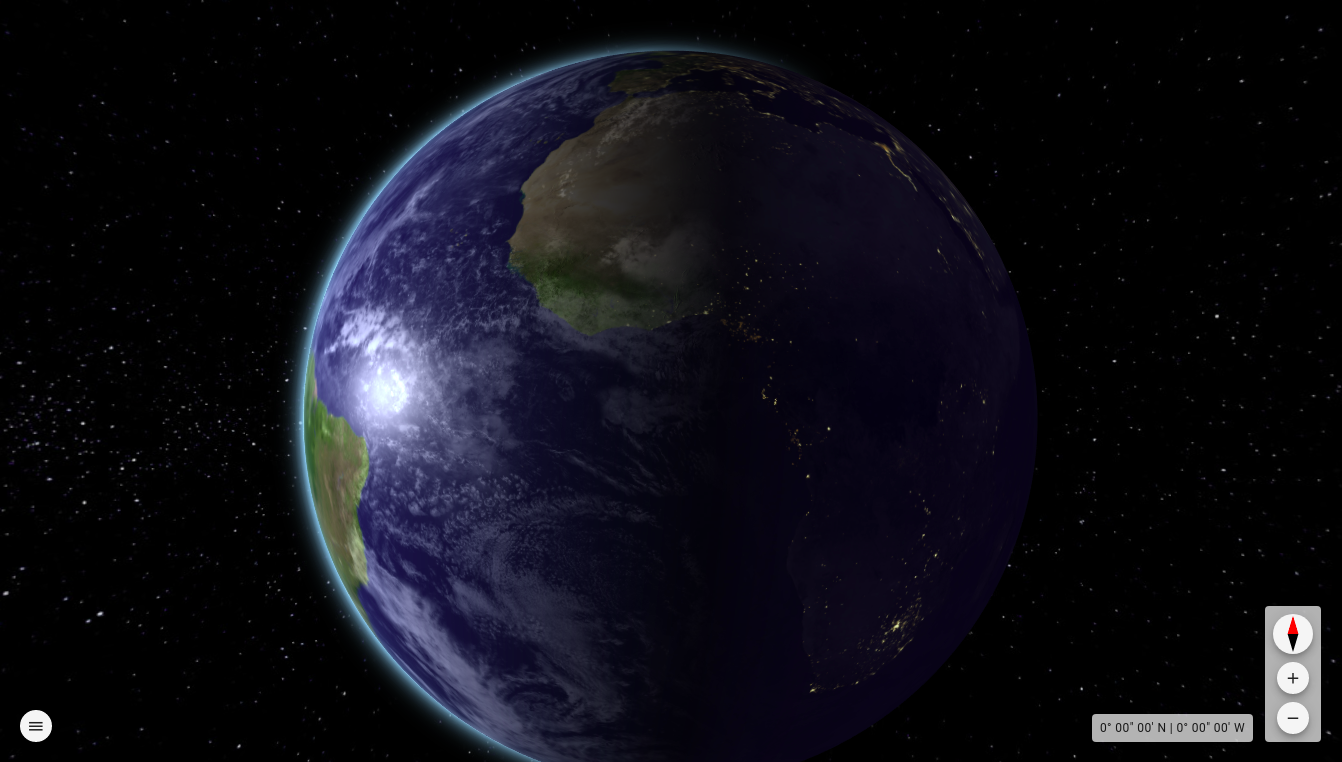
\includegraphics[width=\linewidth]{img/c4_earthVis_1.png}
  \caption{Widok początkowy wizualizacji Ziemi o~godzinie 19:50, 27.09.2020r.}
  \label{fig:c4_earthVis_1} 
\end{figure}
  

\begin{figure}[h]
  \centering
  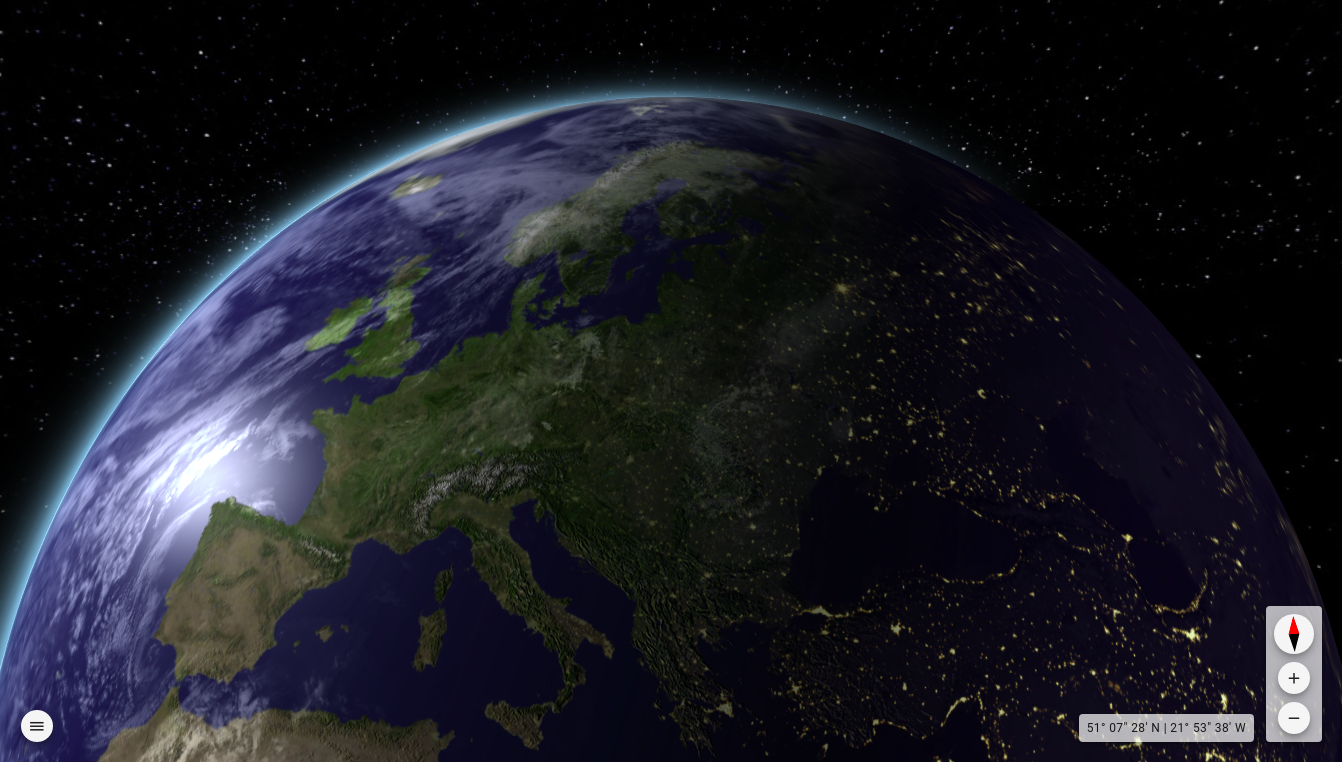
\includegraphics[width=\linewidth]{img/c4_earthVis_2.png}
  \caption{Zachód słońca nad Europą o~godzinie 18:54, 27.07.2020r.}
  \label{fig:c4_earthVis_2} 
\end{figure}
  
Podczas każdej aktualizacji animacji obliczane jest nowe położenie słońca. Poruszając się w~układzie odniesienia Ziemi konieczne jest obliczenie deklinacji Słońca, czyli kąta pomiędzy nim, a~płaszczyzną równika~\cite{Declination}. Drugą wartością konieczną do wyliczenia jest kąt godzinny~\cite{SolarTime}. Jest to kąt, o~jaki obróciło się Słońce od wybranego punktu odniesienia dla wybranej strefy czasowej w~konkretnej chwili. Wizualizacja Ziemi stanowi podstawę do wizualizacji połączonych z~nią zjawisk dużej skali. Bazują na niej wizualizacje \texttt{ActiveSatellitesVis} oraz \texttt{IssVis} opisane w~dalszej części pracy. Na rysunku~\ref{fig:c4_earthVis} przedstawiono diagram zależności pomiędzy poszczególnymi wizualizacjami i~klasami pomocniczymi.

\begin{figure}
  \centering
  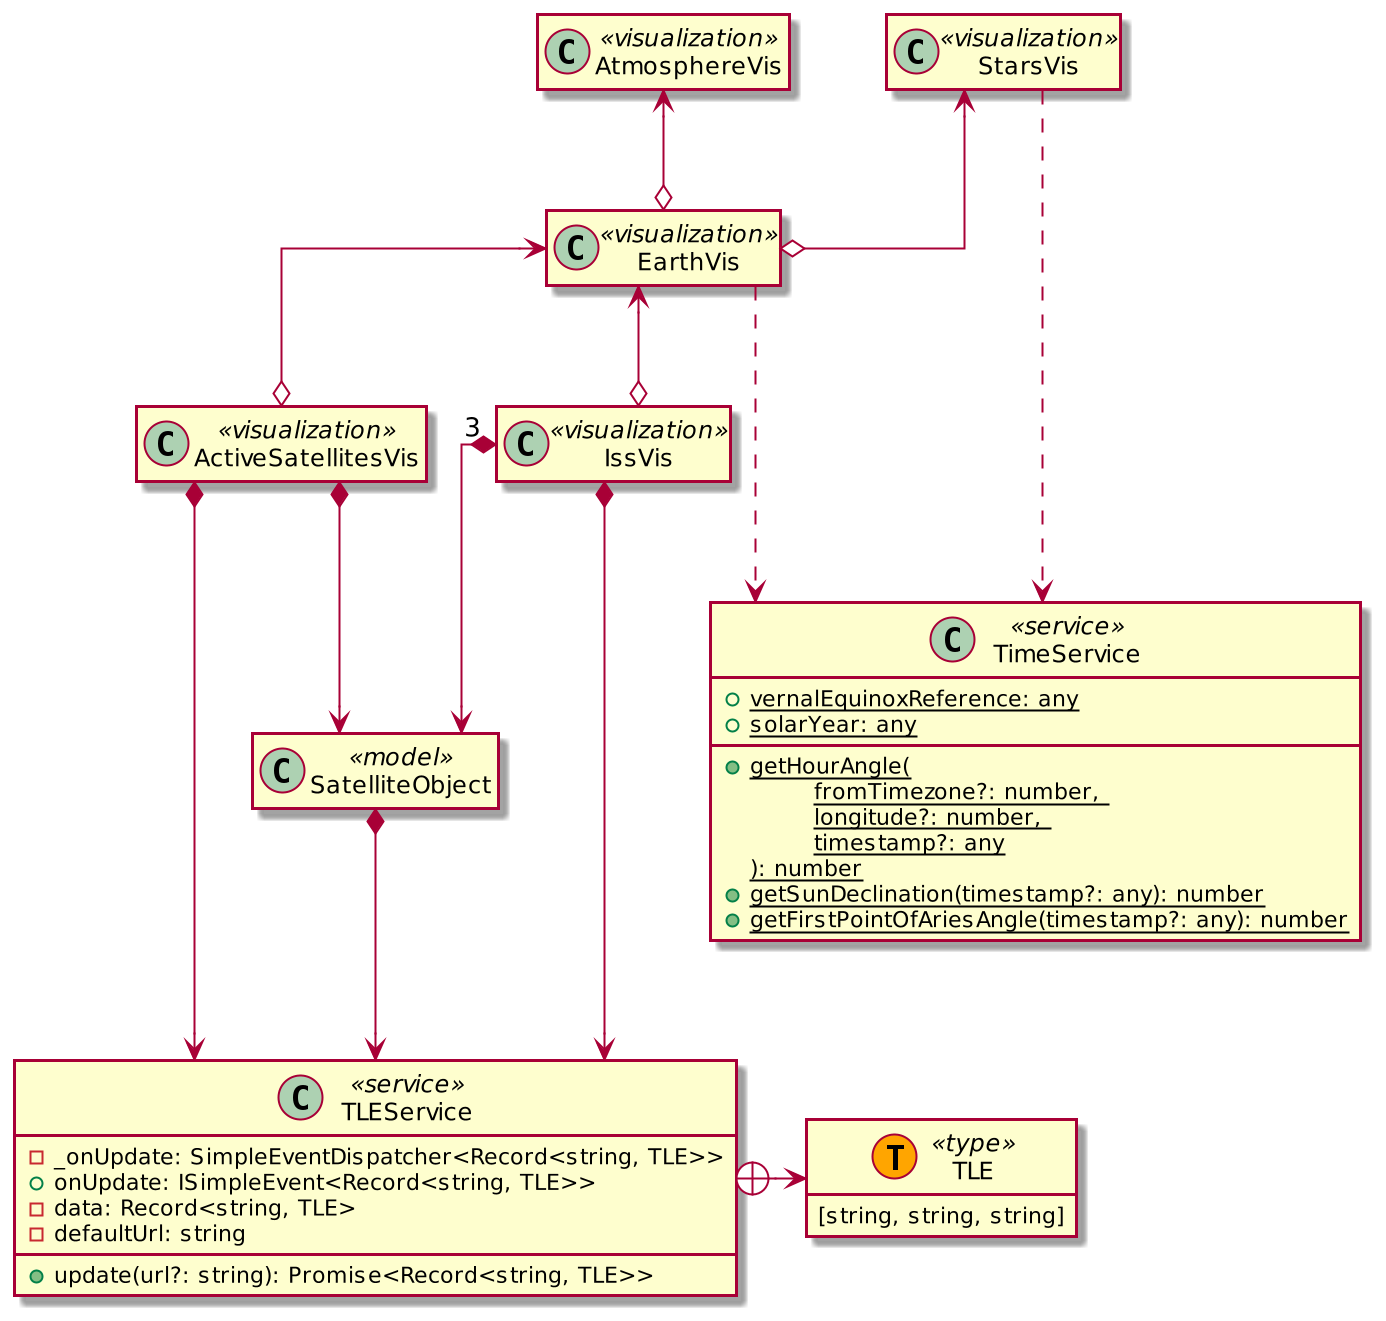
\includegraphics[width=\textwidth]{diagrams/out/c4_earthVis.png}
  \caption{Zależności pomiędzy klasami wizualizacji Ziemi}
  \label{fig:c4_earthVis} 
\end{figure}

Na wizualizację składają się wszystkie obiekty ustawiane przez wizualizacje \texttt{AtmosphereVis} i~\texttt{StarsVis}. Na scenie w~układzie współrzędnych wizualizacji znajdują się dwie sfery. Pierwsza z~nich odpowiada za wyświetlanie tekstury Ziemi, a~druga, z~promieniem większym o~$4$~km, wyświetla chmury. Materiał pierwszej sfery implementuje model oświetlania z~cieniowaniem Phonga~\cite[Rozdział 3]{RealTime3DGraphics} za pomocą obiektu \texttt{THREE.MeshPhongMaterial} i~używa czterech map.
\begin{enumerate}
  \item \texttt{map} - mapa zawierająca kolor tekseli tekstury dziennej
  \item \texttt{nightMap} - mapa zawierająca kolor tekseli tekstury nocnej
  \item \texttt{specularMap} - mapa zawierająca poziom odbicia kierunkowego światła dla każdego teksela tekstury
  \item \texttt{normalMap} - mapa zawierająca wektory normalne w~przestrzeni stycznej wierzchołka modelu.
\end{enumerate}

Materiał sfery wyświetlające chmury zawiera tylko mapę definiującą sam kolor tekseli. Jako, że ta mapa jest obrazem chmur na czarnym tle i~nie zawiera kanału \texttt{alpha}, materiał w~procesie renderowania stosuje mieszanie addytywne. Grupa obrotu zawiera również światło kierunkowe, które zawsze skierowane jest do jej środka. Pozycja źródła światła obracana jest zgodnie z~wartościami wyliczonymi przez serwis \texttt{TimeService}, kolejno o~kąt godzinny w~osi~$OY$ i~deklinację w~osi~$OX$.

Na rysunku~\ref{fig:c4_earthVis_2} pokazane zostało płynne przejście pomiędzy teksturą nocną i~dzienną, która jest wyświetlana w~zależności od oświetlenia planety. Zachowanie to wymagało zmodyfikowania domyślnego fragment shadera i~uzależnienia wyświetlanej tekstury od kąta pomiędzy interpolowanym wektorem normalnym dla teksela, a~kierunkiem padania światła. Na listingu~\ref{lst:earthFrag} pokazano najważniejszą część modyfikacji shadera. Potrzebny kąt wyliczany jest z~wykorzystaniem iloczynu skalarnego wspomnianych wektorów. Wynik ten musi być zmapowany z~przedziału $\lbrack-1; 1\rbrack$ na przedział $\lbrack0; 1\rbrack$. Obliczenie wartości, która trafia do funkcji wygładzającej, a~następnie do funkcji \texttt{mix}, która miesza wartości tekseli, pokazano na równaniu~\ref{eq:earth_dot}.

\begin{lstlisting}[float=h, language=C++, label={lst:earthFrag}, caption={
  Modyfikacja fragment shadera materiału \texttt{MeshPhongMaterial}}
]
#if NUM_DIR_LIGHTS > 0
  float dotL =  dot(vNormal, directionalLights[0].direction);
  vec4 texelColorNight = texture2D( nightMap, vUv );
  texelColorNight = mapTexelToLinear( texelColorNight );

  outgoingLight = mix(
    vec3(texelColorNight) + ambientLightColor,
    outgoingLight,
    easeInOutExpo(dotL*0.5+0.5)
  );
#endif
\end{lstlisting}
\begin{equation}
  \label{eq:earth_dot}
  x = (\vv{n} \cdot \vv{d}) \cdot 0.5 + 0.5
\end{equation}
\begin{eqexpl}[25mm]
\item {$\vv n$} wektor normalny
\item {$\vv d$} kierunek padania światła
\item {$x$} wartość w~przedziale $\lbrack0; 1\rbrack$
\end{eqexpl}
\vspace{\baselineskip}

Wizualizacje dostarcza również panel kontrolny, który pokazany został na rysunku~\ref{fig:c3_controls_earth} i~pozwala na przełączanie się pomiędzy trybami kamery - swobodnym i~kompas.

\section{Wybrane satelity}

Wizualizacją stworzoną na podstawie wizualizacji Ziemi jest wizualizacja wybranych satelitów orbitujących wokół niej. Klasą definiującą tę wizualizację jest klasa \texttt{IssVis} obecna na rysunku~\ref{fig:c4_earthVis}. Znajdują się na nim również klasy wspomagające wyświetlanie i~wyliczanie pozycji obiektów. Na scenie znajdują się trzy satelity. Są nimi Międzynarodowa Stacja Kosmiczna, Kosmiczny Teleskop Hubble'a oraz Eutelsat Hot Bird 13C. Każda satelita reprezentowana jest za pomocą trzech obiektów, którymi jest elipsa reprezentująca kształt orbity, obiekt satelity będący złożonym modelem 3D lub sferą oraz linia łącząca obiekt satelity ze środkiem planety.  Wizualizacja dostarcza komponent panelu kontrolnego, który umożliwia zmianę trybu pracy kamery oraz zarządzenie widocznością poszczególnych satelitów. Pozycja satelitów wyświetlana jest w~czasie rzeczywistym, a~ich pozycja i~orbita kalkulowana jest z~wykorzystaniem danych w~formacie TLE~(ang.~Two-Line Elements).

\subsection{TLE}
TLE jest formatem zapisu informacji o~satelicie pozwalającym wyznaczyć z~dużym przybliżeniem jej pozycję relatywnie do ciała orbitowanego~\cite{TLE}. Pierwsza linia zawiera nazwę satelity i~może być pomijana w~zapisie. Druga linia jednoznacznie identyfikuje satelitę i~zawiera informacje o~punkcie w~czasie, dla którego określone są parametry orbity - epokę. Zawiera również informacje kontrolne o~samym TLE oraz pierwszą i~drugą pochodną prędkości ruchu. Trzecia linia zawiera parametry orbity. Najważniejszymi z~nich są inklinacja, kąt węzła wstępującego, ekscentryczność i~argument perycentrum, który dla Ziemi nazywa się argumentem perygeum. Poniżej przedstawiono przykładowe dane dla Międzynarodowej Stacji Kosmicznej.
\begin{verbatim}
ISS (ZARYA)
1 25544U 98067A   08264.51782528 -.00002182  00000-0 -11606-4 0  2927
2 25544  51.6416 247.4627 0006703 130.5360 325.0288 15.72125391563537
\end{verbatim}

W stworzonej wizualizacji TLE pobierane są ze strony CelesTrak~\cite{CelesTrak}, która zbiera i~analizuje dane otrzymane od jednostki NORAD (ang. North American Aerospace Defense Command). Dane otrzymywane są w~formacie tekstowym. Serwis \texttt{TLEService} odpowiedzialny jest za pobranie danych TLE wszystkich aktywnych satelitów, sparsowanie je, a~następnie wyemitowanie zdarzenia \texttt{onUpdate}, które może być obsłużone w~procesie inicjalizacji obiektów na scenie. Serwis ten umożliwia również dostęp do danych satelity z~wykorzystaniem jej identyfikatora. Dla satelitów, na których pozycję wpływać może atmosfera i~inne nieregularne czynniki, dane TLE mogą z~czasem stawać się nieaktualne. Dzieje się to jednak na przestrzeni dni. Założyć można, że pobranie najnowszej ich wersji w~momencie uruchamiania wizualizacji pozwala na wystarczająco dokładne wyliczenia ich pozycji.

Za obliczenie parametrów orbity, wygenerowanie obiektów sceny i~odpowiednią transformację ich pozycji odpowiada obiekt \texttt{SatelliteObject} reprezentujący pojedynczą satelitę. Oblicza on parametry elipsy i~generuje reprezentujący ją obiekt klasy \texttt{THREE.EllipseCurve}. Równania~\ref{eq:sat_1}~-~\ref{eq:sat_3} opisują proces wyliczenia parametrów orbity. Wyliczenia półosi wielkiej $a$ wynika z~trzeciego prawa Kelpera, które łączy jej długość zależnością z~okresem obiegu satelity wokół Ziemi, który to dostarcza TLE. Transformacja aktualizowana jest w~każdym przebiegu pętli animacji.

\begin{samepage}
  \begin{figure}[h]
  \begin{align}
      \label{eq:sat_1}
      a~&= \frac{G^{\frac{1}{3}}}{(\frac{2n\pi}{86400})^{\frac{2}{3}}} \\
      \label{eq:sat_2}
      b &= a\sqrt{1-e^2} \\
      \label{eq:sat_3}
      c &= e \cdot a
  \end{align}
  \begin{eqexpl}[25mm]
      \item {$a$} półoś wielka orbity
      \item {$G$} standardowy parametr grawitacyjny Ziemi
      \item {$n$} średnia liczba obiegów Ziemi w~ciągu 24 godzin
      \item {$b$} półoś mała orbity
      \item {$e$} ekscentryczność orbity
      \item {$c$} przesunięcie od środka do ogniska orbity
  \end{eqexpl}
  \vspace{\baselineskip}
\end{figure}
\end{samepage}

Finalna transformacja obiektu elipsy jest z~złożeniem obrotów i~translacji. Najpierw wykonywana jest translacja elipsy tak, aby środek Ziemi pokrywał się z~jej ogniskiem. Następnie w~osi $OX$ elipsa obracana jest o~kąt wynikający z~danych o~inklinacji orbity.  Potem wykonywany jest obrót w~osi $OY$ o~kąt wynikający z~położenia punktu Barana, czyli punktu służącego do orientacji w~odniesieniu do równikowego układu współrzędnych oraz ekliptyki. W~tej samej osi elipsa obracana jest o~kąt wynikający z~kąta węzła wstępującego oraz o~kąt przeciwny do kąta godzinnego, aby uwzględnić obrót Ziemi w~czasie. Na końcu następuje obrót uwzględniający argument perygeum. 

Funkcja \texttt{TimeService.getFirstPointOfAriesAngle} odpowiedzialna jest za obliczanie kąta od punktu Barana. W~obecnej implementacji może ona jednak być czynnikiem wpływającym na brak pokrycia orientacji orbity w~osi $OY$ z~jej faktyczną trajektorią. Sztuczna korekcja staje się również nieaktualna po jakimś czasie. Autor wizualizacji nie był w~stanie dostatecznie zbadać przyczyny tego problemu. 

Za obliczanie pozycji samej satelity na orbicie odpowiada biblioteka \texttt{tle.js}~\cite{tle.js}, która jest używana w~procesie aktualizacji obiektu \texttt{SatelliteObject}. Pozwana ona, na postawie TLE, uzyskać położenie satelity o~podanym czasie. Etykiety generowane są z~użyciem obiektu \texttt{THREE.Sprite}, który wyświetla kwadratową teksturę zawsze zorientowaną w~kierunku obserwatora. Tekstura jest napisem, który rysowany jest dynamicznie na elemencie \texttt{Canvas} przetworzonym przez obiekt \texttt{THREE.CanvasTexture}. Rozmiar etykiet jest wprost proporcjonalny do odległości obiektu od obserwatora. Zachowanie to utrzymuje taki sam rozmiar etykiet niezależnie od orientacji kamery na scenie.

\begin{figure}
  \centering
  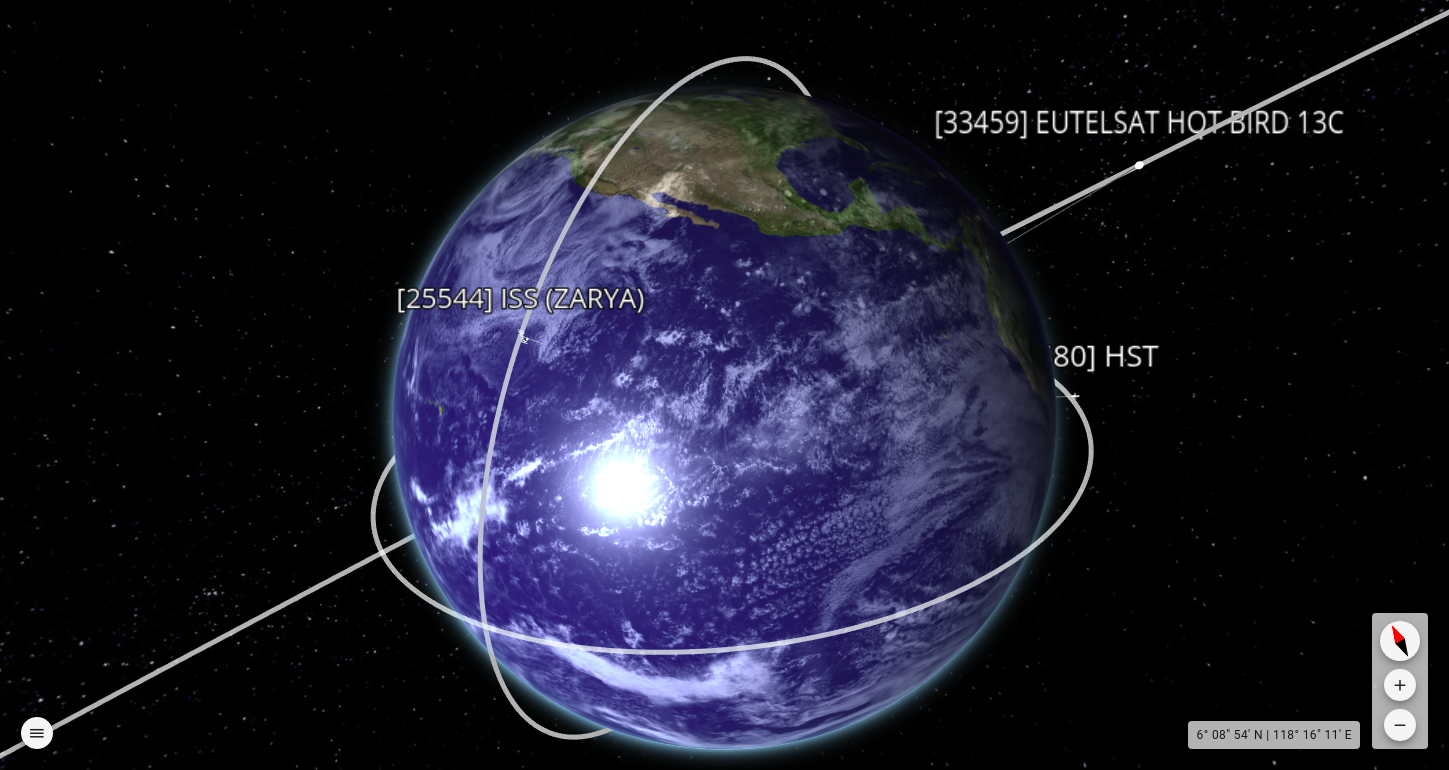
\includegraphics[width=\linewidth]{img/c4_issVis.png}
  \caption{Wybrane satelity - klasa \texttt{IssVis}}
  \label{fig:c4_issVis} 
\end{figure}

\section{Aktywne satelity}

Wizualizacja, którą opisuje klasa \texttt{ActiveSatellitesVis}, która pokazana jest na rysunku~\ref{fig:c4_earthVis}, wyświetla wszystkie aktywne satelity na podstawie danych ze strony CelesTrak~\cite{CelesTrak}. Widok początkowy wizualizacji przedstawia za pomocą punktów pozycje satelitów w~chwili obecnej. Wizualizacja dostarcza panel kontrolny, dzięki któremu można zmienić tryb ruchu kamery oraz przyspieszyć upływ czasu. Można dzięki temu zobaczyć przybliżoną pozycję satelitów w~przyszłości. Panel kontrolny posiada również możliwość resetu czasu wizualizacji do chwili obecnej. Na rysunku~\ref{fig:c4_activeSatellitesVis} pokazana została wizualizacja oraz jej panel kontrolny. Widać na nim dobrze łuk, którą tworzą satelity na orbicie geostacjonarnej.

\begin{figure}
  \centering
  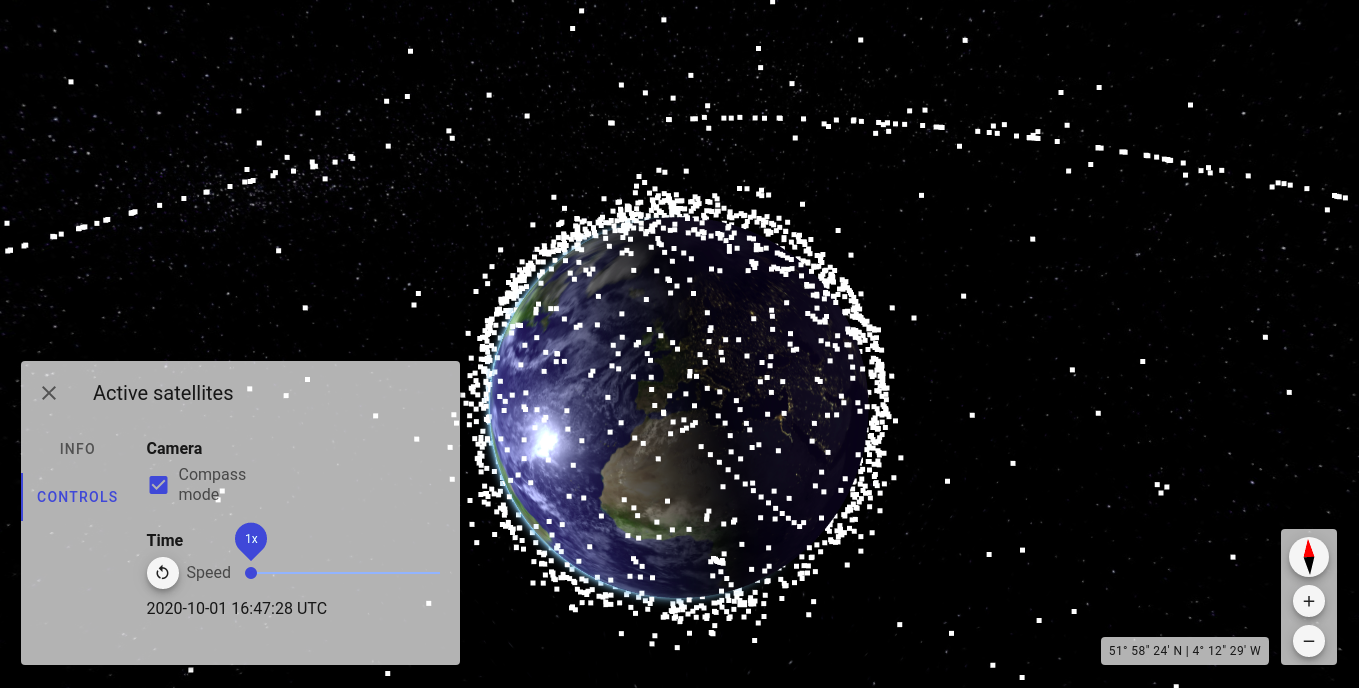
\includegraphics[width=\linewidth]{img/c4_activeSatellitesVis.png}
  \caption{Aktywne satelity - klasa \texttt{ActiveSatellitesVis}}
  \label{fig:c4_activeSatellitesVis} 
\end{figure}

Podobnie jak w~przypadku wizualizacji opisanej klasą \texttt{IssVis} dane TLE pobierane są i~zarządzane poprzez klasę \texttt{TLEService}. Kalkulacja pozycji satelitów również wykonywana jest z~użyciem mechanizmów klasy \texttt{SatelliteObject}. Różnicą pomiędzy tymi wizualizacjami jest to, że klasa \texttt{SatelliteObject} nie tworzy i~nie dodaje do sceny obiektów reprezentujących satelity. 

\begin{lstlisting}[float, language=javascript, label={lst:active1}, caption={
  Fragmenty klasy \texttt{ActiveSatellitesVis}}
]
private pointsMaterial = new THREE.PointsMaterial({
  transparent: true,
  color: 0xffffff,
  size: 5,
  sizeAttenuation: false,
});
private points = new THREE.Points(
  new THREE.BufferGeometry(),
  this.pointsMaterial
);

public update(deltaFrac: number) {
  /* ... */
  const points: number[] = [];
  this.sateliteObjects.forEach((o) => {
    const p = o.getPosition(this.timestamp);
    points.push(p.x, p.y, p.z);
  });
  this.points.geometry.setAttribute(
    "position",
    new THREE.BufferAttribute(new Float32Array(points), 3)
  );
  /* ... */
}
\end{lstlisting}

Dostępne dane zawierają informacje o~około 8000 aktywnych satelitów. Wywołanie polecenia rysowania dla każdego punktu oddzielnie skutkowałoby długim czasem rysowania, ponieważ w~procesie generowania grafiki najwięcej czasu tracone jest na komunikacji z~GPU. Dlatego wizualizacja wywołuje tylko jedno polecenie rysowania dla wszystkich punktów. Listing~\ref{lst:active1} zawiera inicjalizację obiektu materiału \texttt{THREE.PointsMaterial} oraz obiektu \texttt{THREE.Points} odpowiedzialnego za reprezentację punktów na scenie. Inicjalizowany jest on z~pustym buforem reprezentującym pozycje wierzchołków. Rola buforów w~procesie rysowania opisana została w~rozdziale~\ref{sec:render}. W~pokazanej na listingu~~\ref{lst:active1} metodzie \texttt{update}, wykonywanej co każde przejście pętli głównej, bufor uzupełniany jest nowymi współrzędnymi punktów. Wszystkie punkty rysowane są za pomocą jednego polecenia, a~rysowanie każdego z~osobna dzieje się równolegle w~GPU. Największy narzut obliczeniowy spowodowany jest kalkulacją pozycji w~obiektach \texttt{SatelliteObject}, który przy dużych liczbach jest już dostrzegalny.

\section{Kafelki i~Radar pogodowy}

Wizualizacja, którą opisuje klasa \texttt{OsmTiles}, przedstawia Ziemię, na którą nałożono wiele warstw tekstur. Pierwszą z~nich jest mapa przeglądowa powierzchni, drugą jest pokrycie terenu zasięgiem radarów meteorologicznych, a~trzecią z~nich jest wizualizacja danych z~owych radarów w~danej chwili. Szczegółowość mapy zależy od przybliżenia kamery. Wizualizacja składa się z~wcześniej opisanych wizualizacji gwiazd oraz atmosfery. Nie zawiera ona dynamicznego oświetlenia, a~światło kierunkowe znajduje się w~układzie odniesienia obserwatora, zawsze oświetlając widoczną stronę planety.

Panel kontrolny dostarczony przez wizualizację pozwala na zmianę trybu pracy kamery, na zmianę widocznych warstw oraz na zmianę czasu dla wizualizowanych opadów. Wizualizacja pozwala również na animację warstwy opadów, pozwalając na zaobserwowanie ich dynamiki w~ostatnim czasie. Na rysunkach~\ref{fig:c4_osmTilesVis}~oraz~\ref{fig:c4_osmTilesVis_1} przedstawiono mapy w~małej i~średniej skali.
\begin{figure}[h]
  \centering
  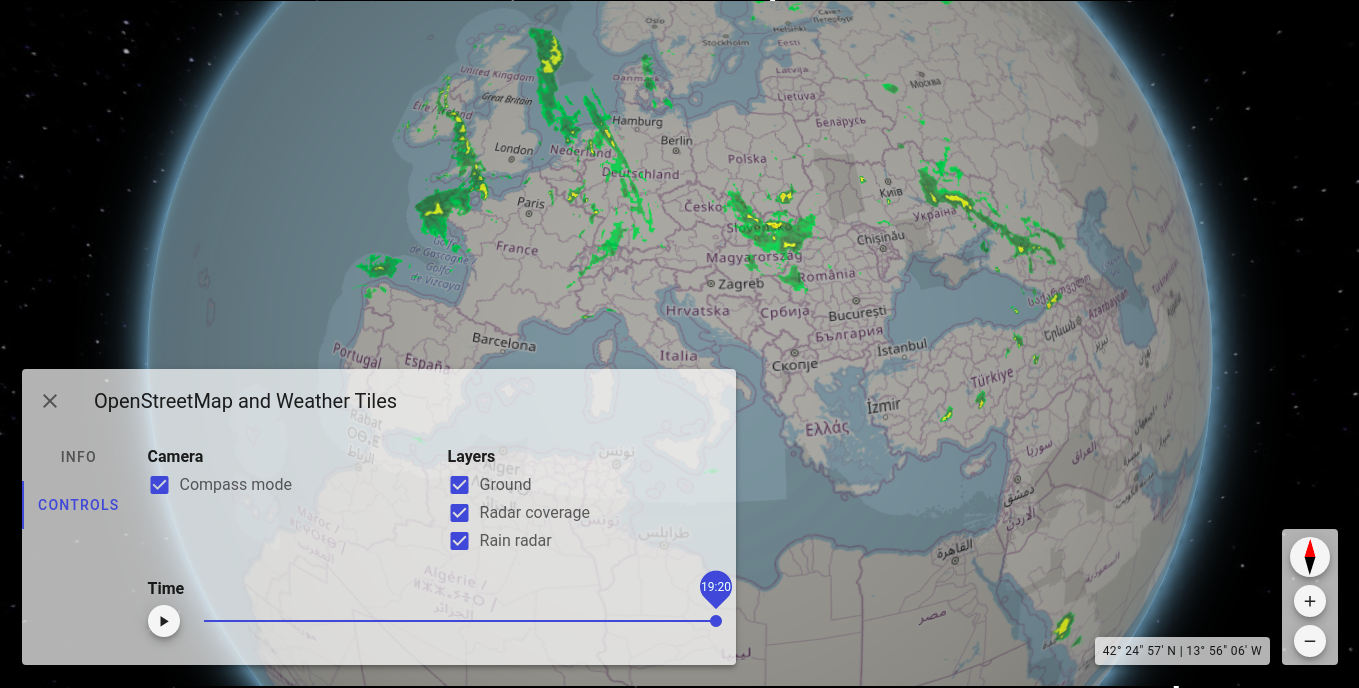
\includegraphics[width=\linewidth]{img/c4_osmTilesVis.png}
  \caption{Opady deszczu nad Europą - klasa \texttt{OsmTilesVis}}
  \label{fig:c4_osmTilesVis} 
\end{figure}

\begin{figure}[h]
  \centering
  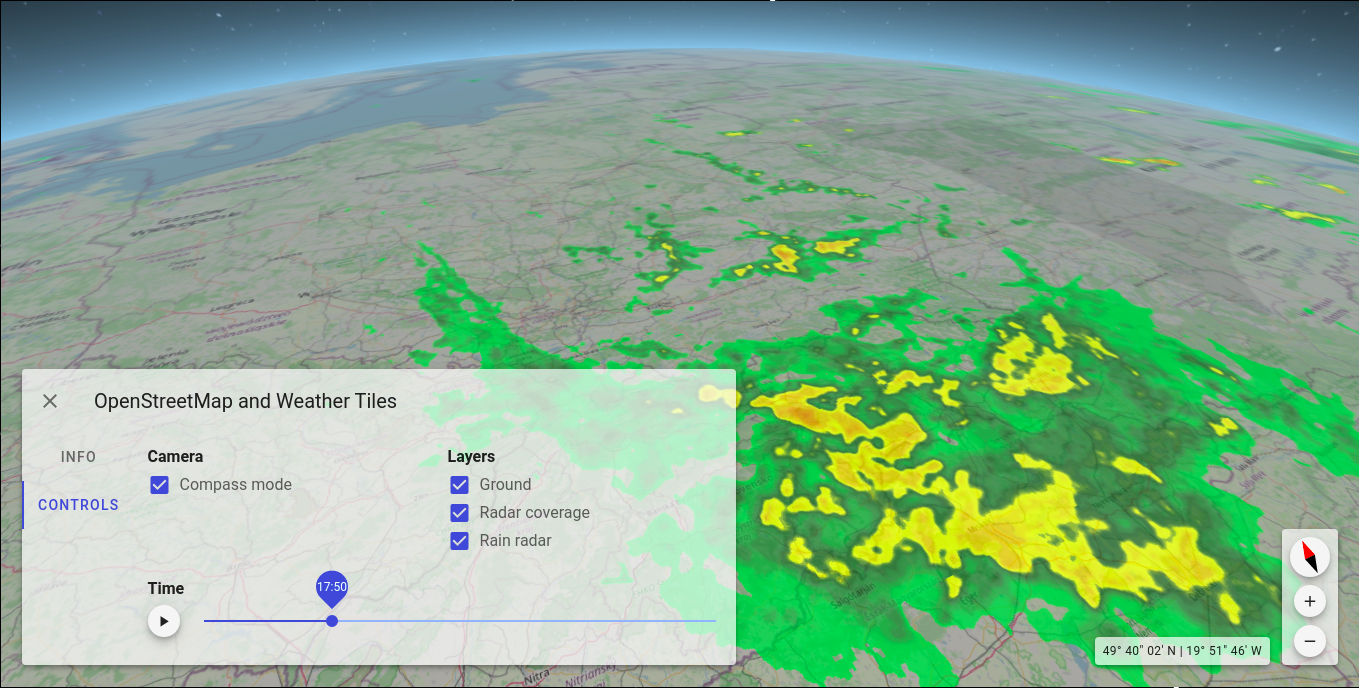
\includegraphics[width=\linewidth]{img/c4_osmTilesVis_1.png}
  \caption{Opady deszczu nad Polską - klasa \texttt{OsmTilesVis}}
  \label{fig:c4_osmTilesVis_1} 
\end{figure}

\subsection{Kafelki}
Kafelki są sposobem reprezentacji danych mapy. Pozwalają na optymalizację jej wyświetlania, ponieważ dzielą obszar na niezależne fragmenty, z~których można skomponować pożądany widok. Dzięki nim można pobierać te dane, które aktualnie są potrzebne. Kafelki mogą być dowolnymi danymi, które mapują pewne wartości na powiązane z~nimi pozycje na mapie. W~przypadku opisu wyglądu obiektów na mapie mogą występować w~postaci grafiki wektorowej jak i~rastrowej.

W celu odwzorowania powierzchni Ziemi na płaską grafikę zaszła potrzeba dobrania odpowiedniej metody jej projekcji. Odwzorowanie walcowe równokątne, zwane odwzorowaniem Merkatora jest metodą projekcji, w~której kąty pomiędzy równoleżnikami i~południkami są zachowane. Wszystkie południki na mapie są równoległe do siebie, a~co za tym idzie, odwzorowanie to na biegunach dąży do nieskończoności. Web Merkator~\cite{Mercator} to modyfikacja odwzorowania Merkatora wykorzystywana przez zdecydowaną większość map dostępnych w~internecie. Od swojego pierwowzoru różni się tym, że obszar mapowany jest na powierzchni sfery, a~nie tak jak pierwotnie, na elipsoidzie. Projekcja ta nie odwzorowuje też terenu dla szerokości geograficznej większej od~$\ang{85.051129}$. Pozwala to na umieszczenie odwzorowanego terenu na kwadratowej powierzchni. Pojedynczy kafelek rastrowy zwykle jest kwadratem o~boku $256$ pikseli.

Kafelki generowane są dla różnych poziomów szczegółowości, co skutkuje różną wymaganą do ich wyświetlenia rozdzielczością przyjmując ten sam punkt odniesienia. Aby zachować stały rozmiar kafelka, kolejne poziomy szczegółowości zawierają odpowiednio więcej kafelków. Aby ujednolicić poruszanie się po kafelkach wprowadzono system współrzędnych, który jednoznacznie identyfikuje kafelek. Powiązanie kafelków ze współrzędnymi geograficznymi ich lewego górnego rogu opisane zostało za pomocą równań~\ref{eq:tile_1}~-~\ref{eq:tile_2}. Z~równań tych wynika, że dla przybliżenia $z = 0$ mapa składa się z~jednego kafelka. Liczba kafelków $n$, z~których składa się mapa, w~zależności od przybliżenia $z$ opisana może zostać zależnością $n = 2^{2z}$.

\begin{samepage}
  \begin{figure}[h]
  \begin{align}
      \label{eq:tile_1}
      x &= \left\lfloor \frac{lon + 180}{360} \cdot 2^z \right\rfloor \\
      \label{eq:tile_2}
      y &=
          \left\lfloor
              \left(
                  1 - \frac{
                      \ln \left(
                          \tan \left(
                              lat \cdot \frac{\pi}{180}
                          \right) + \frac{1}{\cos \left( lat \cdot \frac{\pi}{180} \right)}
                      \right)
                  }{\pi}
              \right) \cdot 2^{z - 1}
          \right\rfloor
  \end{align}
  \begin{eqexpl}[25mm]
      \item {$x$} pozycja odpowiadająca długości geograficznej
      \item {$lon$} długość geograficzna w~stopniach
      \item {$y$} pozycja odpowiadająca szerokości geograficznej
      \item {$lat$} szerokość geograficzna w~stopniach
      \item {$z$} stopień szczegółowości (przybliżenia)
  \end{eqexpl}
  \vspace{\baselineskip}
\end{figure}
\end{samepage}

\subsection{Implementacja}

Wizualizacja, pobierając potrzebne dane kafelków, korzysta z~domyślnego zestawu warstw map OpenStreetMap~\cite{OSM}. Dane dotyczące radaru i~deszczu udostępniane są przez aplikację RainViewer~\cite{RainViewer}. Kafelki z~obu tych źródeł udostępniane są w~tym samym, pożądanych formacie. Na diagramie na rysunku~\ref{fig:c4_tiles} przedstawiono klasę \texttt{TilesService} oraz jej zależności, która odpowiedzialna jest za generowanie i~zarządzanie geometrią sceny związanej z~kafelkami. Wywołanie konstruktora tej klasy, pokazane na listingu~\ref{lst:tilesVis_1}, zawiera przekazany obiekt konfiguracji, który zawiera metodę zwracającą adres URL kafelka dla pożądanej pozycji i~przybliżenia, ustawienie widoczności i~filtry CSS, modyfikujące oryginalny wygląd pobranej grafiki.

\begin{figure}[h]
  \centering
  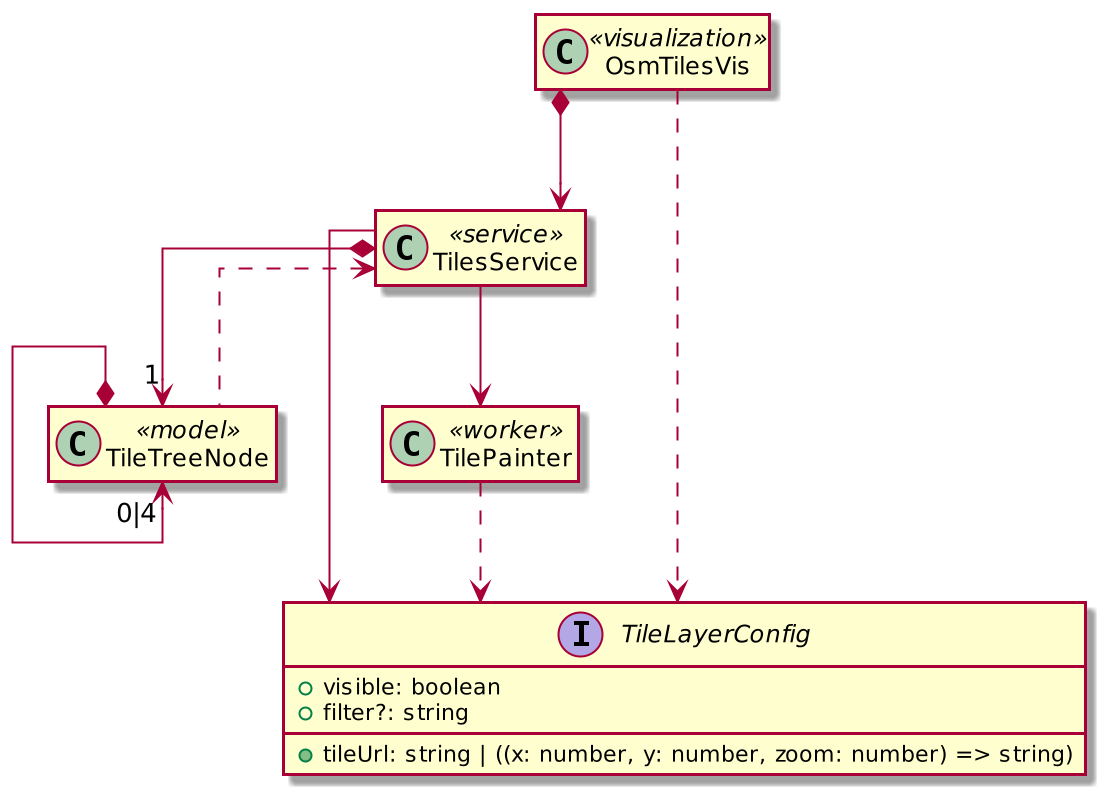
\includegraphics[scale=0.7]{diagrams/out/c4_tiles.png}
  \caption{Zależności pomiędzy klasami wizualizacji \texttt{OsmTilesVis}}
  \label{fig:c4_tiles} 
\end{figure}

\begin{lstlisting}[float=h, language=javascript, label={lst:tilesVis_1}, caption={
  Fragmenty klasy \texttt{OsmTilesVis}}
]
/* ... */
this.osmTilesService = new TilesService(
    [
      {
        tileUrl: (x, y, z) =>
          `https://tile.openstreetmap.org/${z}/${x}/${y}.png`,
        visible: true,
        filter: "brightness(60%)",
      },
      {
        tileUrl: (x, y, z) =>
          `https://tilecache.rainviewer.com/v2/coverage/0/256/${z}/${x}/${y}.png`,
        visible: true,
        filter: "opacity(10%)",
      },
      {
        tileUrl: (x, y, z) =>
          `https://tilecache.rainviewer.com/v2/radar/${
            this.timestamps[this.timestampIndex]
          }/256/${z}/${x}/${y}/4/1_1.png`,
        visible: true,
        filter: "opacity(60%)",
      },
    ],
    100
  );
/* ... */
\end{lstlisting}

Każdy kafelek jest wycinkiem sfery, za którego utworzenie odpowiada konstruktor klasy \texttt{THREE.SphereGeometry}. Wygenerowana geometria może być współdzielona dla każdego kafelka na tej samej szerokości geograficznej i~z tym samym przybliżeniem, dlatego serwis \texttt{TileService} zapisuje raz wygenerowaną geometrię do map, których kluczami są współrzędne~$y$~i~$z$ kafelków. W~przypadku ponownego użycia kafelków dla tych współrzędnych ich geometria pobierana jest z~mapy. Serwis ten definiuje również metody przeliczające długość i~szerokość geograficzną na współrzędne~$x$~i~$y$ dla określonego przybliżenia $z$. Definiuje też przekształcenie odwrotne.

Kafelki tworzą strukturę drzewiastą. Korzeniem drzewa jest kafelek o~współrzędnych $(x, y, z) = (0,0,0)$. Po zwiększeniu przybliżenia dzielony jest on na cztery mniejsze kafelki o~współrzędnych $(0,0,1)$, $(1,0,1)$, $(0,1,1)$ i~$(1,1,1)$. Każdy kafelek w~drzewie może posiadać czterech potomków. Drzewo kafelków rozwijane jest w~sposób możliwie optymalny, a~wyświetlane są zawsze kafelki będące liśćmi tego drzewa. Nie ma potrzeby rozwijać poddrzewa kafelków dla obszaru będącego po drugiej stronie planety, ponieważ nie jest on widoczny. Nie ma również potrzeby wyświetlania kafelków wysokiej rozdzielczości na horyzoncie, ponieważ znajdując się daleko, wyświetlane są one z~użyciem mniejszej ilości pikseli, a~co za tym idzie, wymagają mniejszej dokładności. Serwis \texttt{TilesService} zawiera instancję klasy \texttt{TileTreeNode} reprezentującej węzeł drzewa, który w~tym przypadku jest jego korzeniem. Węzeł drzewa odpowiedzialny jest za generowanie swoich potomków oraz niszczenie samego siebie i~rysowanie swojej tekstury.

Drzewo analizowane jest pod kątem pożądanego stopnia szczegółowości $z$. W~rekurencyjnym rozwijaniu drzewa brana jest pod uwagę odległość kafelka od kafelka, nad którym znajduje się kamera w~metryce taksówkowej na tym samym poziomie szczegółowości oraz kąt pod jakim kamera spogląda na kafelek. Im większa owa odległość i~kąt, tym rozwijanie kafelków zakończy się wcześniej, nie osiągając danego stopnia $z$ w~obszarach, które nie są ważne z~perspektywy generowanego widoku. Działanie to jest główną metodą optymalizacji wyświetlanych kafelków. Rozwinięte wcześniej węzły drzewa, których stopień szczegółowości jest większy niż pożądany, są niszczone. Przykładowe rozwinięcie węzłów drzewa pokazano na diagramie na rysunku~\ref{fig:c4_tilesTree}. Liście oznaczone kolorem czerwonym są wyświetlane. Działanie w~praktyce zaobserwować można na rysunku~\ref{fig:c4_osmTilesVis_custom}, gdzie wszystkie kafelki zawierają grafikę z~ich współrzędnymi. Na horyzoncie widać wyświetlane kafelki z~mniejszym poziomem szczegółowości. 

\begin{figure}[h]
  \centering
  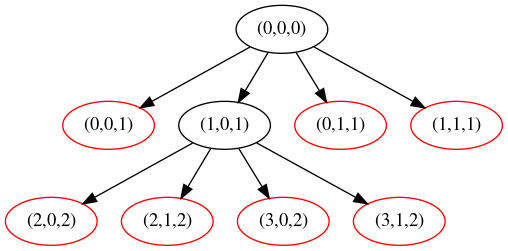
\includegraphics[scale=0.5]{diagrams/out/c4_tilesTree.png}
  \caption{Przykładowe rozwinięcie drzewa kafelków}
  \label{fig:c4_tilesTree} 
\end{figure}

\begin{figure} 
  \centering
  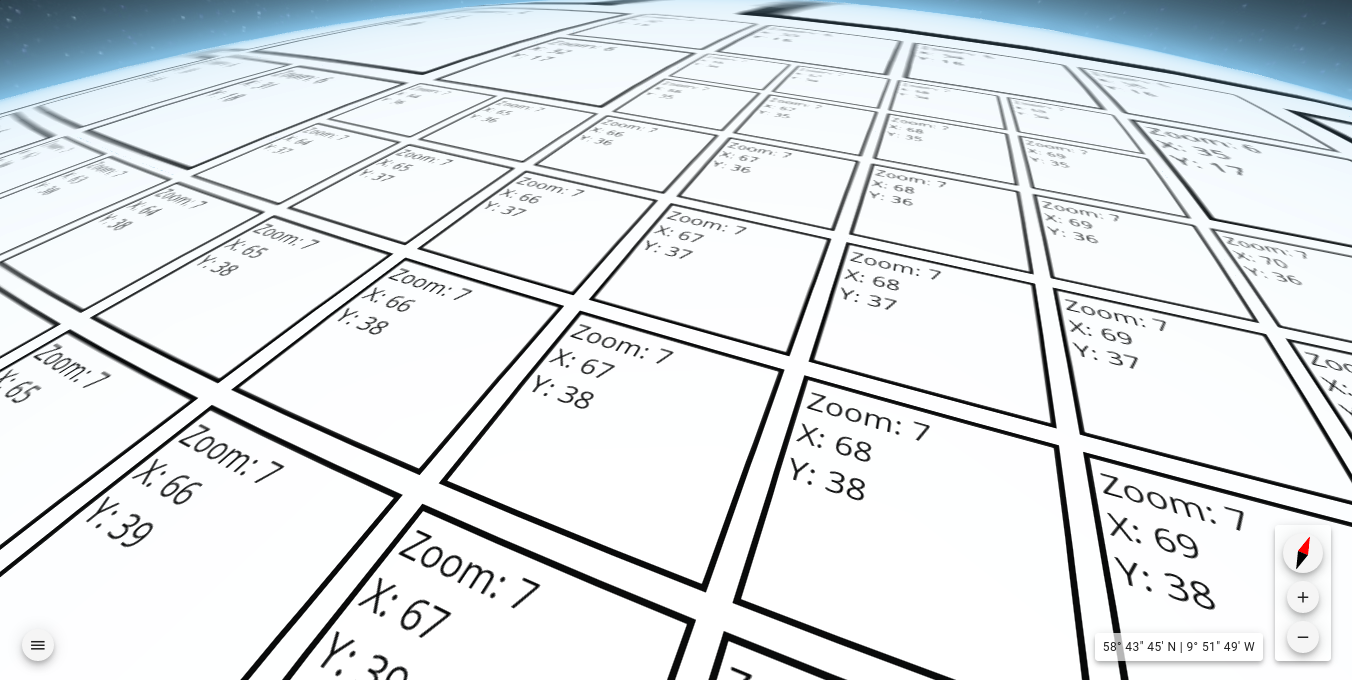
\includegraphics[width=\linewidth]{img/c4_osmTilesVis_custom.png}
  \caption{Rozwinięcie drzewa kafelków - testowe kafelki}
  \label{fig:c4_osmTilesVis_custom} 
\end{figure}

Na obiekt kafelka w~procesie rysowania nałożona zostaje dynamicznie tekstura. Pochodzi ona z~obiektu \texttt{Canvas}, który obsługiwany jest przez obiekt \texttt{THREE.CanvasTexture}. Pobieranie obrazów, ich późniejsze dekodowanie i~późniejsza kompozycja warstw w~jedną teksturę kafelka wymaga pewnej mocy obliczeniowej. Przy mapie złożonej z~dużej liczby kafelków czynności te, jeśli zajmowałby się nimi wątek główny JavaScriptu, mogą stanowić obciążenie dla urządzenia wyświetlającego wizualizację. Kod wykonujący się domyślnie w~przeglądarce internetowej może wykonać się tylko w~jednym wątku. Aby wprowadzić możliwość akceleracji obliczeń dla zadań, które mogą wykonywać się w~tle i~nie mają nic wspólnego z~interfejsem użytkownika, stworzone zostały Web~Workery~\cite{Workers}. Aby rozwiązać problem bezpieczeństwa w~komunikacji pomiędzy wątkami, workery korzystają ze ściśle określonego interfejsu. Nie współdzielą one między sobą pamięci, którą można przekazywać jedynie w~jedną stronę poprzez operację transferu. Sama komunikacja opera się na zdarzeniach, których dane są serializowane i~deserializowane na styku wątków. Aby odciążyć główny wątek w~procesie rysowania sceny, operacje pobierania i~kompozycji kafelków odbywają się w~workerze, czyli całkowicie niezależnie od głównej pętli animacji.

Klasa \texttt{TilePainter} reprezentuje obiekt workera. Standardowy obiekt \texttt{Canvas} jest elementem DOM, do którego nie ma dostępu w~workerach, ponieważ nie kontrolują one interfejsu użytkownika. Na potrzeby rysowania grafik w~tle zaproponowano interfejs \texttt{OffscreenCanvas}~\cite{OffscreenCanvas}, który zachowuje się dokładnie tak jak element \texttt{Canvas} dostępny w~głównym wątku.

Kiedy użytkownik zmieni widoczność warstwy lub przesunie kamerę pokazując nowe kafelki, wywołane zostają zdarzenia, które po przejściu przez mechanizm \texttt{throttle} wywołują przeliczenie drzewa kafelków. Każdy kafelek, jeśli nigdy nie miał wygenerowanej tekstury lub jeśli wymagania co do wyglądu tekstury uległy zmianie, wysyła, poprzez serwis \texttt{TilesService}, zdarzenie do workera \texttt{TilePainter}. Następnie worker pobiera wymagane kafelki z~ich źródeł i~nakłada je na siebie wykorzystując zdefiniowane filtry. W~zdarzeniu zwrotnym obiekt bitmapy zostaje przetransferowany do wątku głównego i~tam narysowany na elemencie \texttt{Canvas} tekstury z~użyciem szybkiego kontekstu \texttt{bitmaprenderer}. Worker, w~celu zaoszczędzenia pamięci i~transferu sieciowego, prowadzi cache już narysowanych kafelków i~omija proces pobierania i~kompozycji, jeśli kafelek został już wcześniej przetworzony.

Obiekty wygenerowanej geometrii wycinków sfer reprezentujących kafelki są przekształcane po wygenerowaniu. Obiekt przesuwany jest tak, że jego centroid znajduje się w~środku układu współrzędnych. Następnie, w~definiowanej dla niego macierzy przekształcenia, oprócz obrotu o~kąt wynikający z~długości geograficznej kafelka, to przesunięcie jest odwracane. Działanie to ma na celu zniwelowanie efektu zatracenia precyzji w~procesie przetwarzania wierzchołków przez procesor graficzny. Wierzchołki zdefiniowane daleko od środka układu współrzędnych obarczone są większym błędem związanym z~funkcjonowaniem liczb zmiennoprzecinkowych. Rozmiar liczby dla typu \texttt{Number} w~języku JavaScript wynosi 64b, a~procesor graficzny standardowo przetwarza współrzędne zapisane za pomocą liczb o~rozmiarze 32b. Dla większych liczb, w~procesie wyliczania finalnej pozycji wierzchołka, występuje zanik precyzji spowodowany operacją mnożenia. Zdecydowanie lepiej zdefiniować obiekt z~pozycją blisko środka układu współrzędnych, przekształcić go, a~następnie wykonać translację na jego finalną pozycję. Translacja, jako operacja dodawania, nie zaburza precyzji.

\section{Podsumowanie}

Wizualizacje opisane wcześniej i~obecne jako przykłady w~komponencie Silnika są prezentacją możliwości, jakich dostarcza zaproponowany przez projekt sposób definicji wizualizacji. Opisanie wizualizacji przez pojedynczą klasę, która rozszerza klasę bazową z~dobrze udokumentowanym interfejsem pozwala na bezpośrednią ingerencję kodu w~kształt sceny. System, będąc z~założenia systemem wyświetlającym scenę trójwymiarową, może być użyty do definiowania wizualizacji hybrydowych, gdzie dane z~warstw 2D mogą być nakładane i~wyświetlane na trójwymiarowej powierzchni~\cite{Hybrid}. Atrakcyjna prezentacja danych powiązanych z~punktami na mapie może również obejmować generowanie trójwymiarowych wykresów.

Łatwo konfigurowalny panel kontrolny wykorzystywany może być do sterowania wyglądem wizualizacji. Przez bezpośrednie połączenie z~interfejsem sterowania kamerą, jak i~samą wizualizacją, może być używany do pokazywania i~ukrywania warstw danych, do zmiany położenia kamery, czy do sterowania animacją upływu czasu dla wizualizowanych zjawisk. Przykładem może być dynamika wzrostu zachorowań na COVID-19, czy też zobrazowanie wzorców przemieszczania się ludzi dla różnych pór dnia~\cite{Kwan}.

Oddanie pełnej kontroli nad wizualizacją daje możliwość swobodnej optymalizacji wyświetlanej sceny, a~mechanizmy przetwarzania danych w~innym wątku, oraz asynchroniczne pobieranie niezbędnych zasobów daje możliwość operacji na wielkich zbiorach danych wyświetlając jedynie interesujące odbiorcę w~danej chwili fragmenty z~odpowiednią precyzją, mając na uwadze, że grafika generowana jest w~środowisku przeglądarki internetowej. Z~dużymi możliwościami przychodzi jednak duża odpowiedzialność. To od twórcy zależy jak jego wizualizacja będzie się zachowywać w~kontekście wydajności i~interakcji z~użytkownikiem.

Komponent Silnika, definiując tylko zachowanie kamery i~podstawowe założenia definicji wizualizacji pozwala na utworzenie kolejnych warstw abstrakcji. Możliwe jest na przykład utworzenie w~pełni konfigurowalnego systemu wyświetlającego dane dostarczone w~postaci kafelków, który jest dużo bardziej zaawansowany niż ten opisany w~przykładowej wizualizacji. Może obsługiwać on wiele formatów kafelków, rastrowe oraz wektorowe. Może również pozwalać na nałożenie warstw trójwymiarowych, na dodanie interesujących statystyk w~postaci wykresów lub etykiet, czy też na morphing kafelków dla danych w~czasie. Wszystko sprowadza się do stworzenia przetestowanego podsystemu, który będzie udostępniony i~wykorzystany przez innych twórców. 
% \include{chapter02}
% \include{chapter03}
% \include{chapter04}
% \include{chapter05}
% \include{chapter06}

%\bibliographystyle{plalpha}
\bibliographystyle{abbrv}
% \bibliographystyle{plain}

%Warning: References should be collected in a separate file. You can use the programm JabRef for editing. 
%         But please remember, that not all JabRef types of entries are supported by BibTeX.
%         File name below is given without extenion 
%         (here BibTeX will look for "bibiography.bib" in the main directory)
\setlength{\bibitemsep}{2pt} % introduced to make smaller seps between bibliographic items
\bibliography{bibliography}

%\appendix
%\chapter{Opis załączonej płyty CD/DVD}
Dołączona płyta zawiera wszystkie pliki wykorzystane do stworzenia projektu, dokumentacji i~niniejszej pracy. Pliki podzielono na następujące katalogi:

\begin{enumerate}
    \item \texttt{.vscode} - ustawienia środowiska VsCode,
    \item \texttt{app} - kod źródłowy Aplikacji,
    \item \texttt{docs} - notatki oraz treść i materiały niniejszej pracy,
    \item \texttt{engine} - kod źródłowy i dokumentacja komponentu Silnika,    \item \texttt{testTileService} - kod źródłowy testowego serwisu generującego kafelki.
\end{enumerate}
%\include{appendixB}

%%Uncomment the lines below, if you want to use index
%%\chapterstyle{noNumbered}
%%\phantomsection 
%%\addcontentsline{toc}{chapter}{Index}
%%\printindex


\end{document}